\documentclass[journal]{IEEEtran}

% ===== Idioma y codificación =====
\usepackage[utf8]{inputenc}
\usepackage[T1]{fontenc}
\usepackage[spanish,es-tabla]{babel}
\usepackage{lmodern}
\usepackage{float}

% ===== Gráficos y tablas ===== 
\usepackage{graphicx}
\graphicspath{{figuras/}{figuras/capturas/}}
\usepackage{booktabs}
\usepackage{array}
\usepackage{multirow}

% ===== Matemáticas =====
\usepackage{amsmath,amssymb}
\usepackage{siunitx}

% ===== Código fuente =====
\usepackage{listings}
\usepackage{xcolor}
\lstset{
  basicstyle=\ttfamily\footnotesize,
  keywordstyle=\color{blue!70!black}\bfseries,
  commentstyle=\color{green!50!black}\itshape,
  stringstyle=\color{red!70!black},
  numbers=left, numberstyle=\tiny\color{gray},
  frame=single, breaklines=true, tabsize=2,
  showstringspaces=false, captionpos=b
}

% ===== Referencias cruzadas y URLs =====
\usepackage{url}
\usepackage[hidelinks]{hyperref}
\usepackage{cleveref}

% ===== Bibliografía =====
% Opción A: BibTeX (se configura abajo, al final del documento)
% Si más adelante quieres usarlo, ya está listo.

% ===== Metadata del documento =====
\title{GOATGuard: Sistema de Monitoreo de Infraestructura \\
       y Gestión de Seguridad con Acceso Móvil}

\author{Juan Pablo Carvajal Giraldo,
        Juan David Monsalve Niño,
        y Johan David Rodríguez Castro
\thanks{Los autores pertenecen a la Facultad de Ingeniería de Sistemas 
e Informática de la Universidad Pontificia Bolivariana, Seccional 
Bucaramanga, Colombia.}
\thanks{Proyecto Integrador III, dirigido por el docente Omar Pinzón Ardila.}
\thanks{Bucaramanga, abril de 2026.}}

\markboth{Proyecto Integrador III --- 2026}%
         {Carvajal, Monsalve, Rodríguez: GOATGuard}

\begin{document}

\maketitle

\begin{abstract}
La gestión de infraestructura en redes de área local enfrenta una 
limitación estructural, en donde los modelos convencionales de monitoreo 
dependen de consolas estáticas ancladas a estaciones de trabajo 
fijas, carecen de mecanismos de captura distribuida a nivel de 
endpoint, y no transforman los datos crudos de red en información 
contextualizada por dispositivo, lo que prolonga los tiempos de 
detección de anomalías y deja fuera del inventario a los 
dispositivos no autorizados. Este trabajo presenta el diseño, la 
implementación y la validación de GOATGuard, un sistema de 
monitoreo de redes LAN que articula sensores de captura 
desplegados en los endpoints, un backend centralizado organizado 
según el patrón Pipes and Filters, un motor de detección de 
anomalías basado en medias móviles ponderadas exponencialmente con 
Z-Score adaptativo y filtro de persistencia, y una aplicación 
móvil conectada al servidor mediante una red privada que permite 
el acceso remoto sin exposición a Internet. El diseño se fundamenta 
en el modelo de referencia IPFIX de la IETF y en los estándares del 
modelo OSI, e incorpora decisiones explícitas de sanitización del 
tráfico alineadas con el marco legal colombiano de protección de 
datos personales. La validación funcional se realizó en un entorno 
controlado de catorce nodos con doce endpoints instrumentados, y 
caracterizó la huella del sistema en un régimen de operación 
continua. El trabajo documenta no solo un sistema funcional sino el 
conjunto de decisiones arquitectónicas y normativas que su 
construcción exigió, y deja planteadas líneas específicas de 
extensión hacia detección multivariada y validación de seguridad.
\end{abstract}


\begin{IEEEkeywords}
monitoreo de red, captura distribuida, detección de anomalías,
EWMA, inventario dinámico, aplicación móvil, IPFIX, RUP, OSI, LAN.
\end{IEEEkeywords}

\IEEEpeerreviewmaketitle

% ===== Cuerpo del documento =====
\section{Introducción}
Las redes constituyen la base operativa sobre la cual las 
organizaciones sostienen sus procesos de comunicación y acceso a la 
información. Mantener la visibilidad sobre lo que ocurre dentro de estas 
redes es una condición necesaria para preservar la disponibilidad de los 
servicios y la seguridad de los activos conectados. Sin embargo, las 
herramientas de monitoreo tradicionales operan desde un punto fijo 
mediante puertos mirror o interfaces observadas
~\cite{kurose2010redes}, lo que ofrece una visión agregada del tráfico 
pero carece de granularidad por dispositivo, y obliga al administrador 
a permanecer anclado a una estación de trabajo para consultar esa 
información. Cualquier desplazamiento genera un intervalo sin vigilancia 
durante el cual la red sigue operando pero nadie observa su 
comportamiento.

El presente trabajo aborda esta problemática mediante el desarrollo de 
GOATGuard, un sistema de monitoreo distribuido con acceso móvil 
compuesto por tres componentes: un sensor de captura desplegable en 
cada endpoint de la red, un backend centralizado que recibe, procesa y 
almacena la información reportada por los sensores, y una aplicación 
móvil desde la cual el administrador consulta el estado de la red y 
recibe notificaciones ante comportamientos inusuales. Los sensores 
capturan el tráfico directamente en el endpoint donde operan, lo que 
permite correlacionar cada flujo de red con el dispositivo que lo 
originó sin exponer el contenido del payload~\cite{stevens2004unix}. 
El backend delega la inspección profunda de protocolos al framework 
Zeek~\cite{paxson1999zeek} y aplica un motor de detección de anomalías 
basado en media móvil ponderada exponencialmente con Z-Score adaptativo 
~\cite{hunter1986ewma}, capaz de construir un perfil individual por 
dispositivo sin recurrir a umbrales fijos ni a modelos de aprendizaje 
automático externos.

El aporte del proyecto no reside en la introducción de una técnica 
aislada, sino en la integración de captura distribuida, procesamiento 
contextualizado, inventario dinámico de activos y acceso móvil fuera 
de una arquitectura unificada, orientada a redes de pequeña y mediana 
escala donde las alternativas comerciales resultan económicamente 
inviables u operativamente sobredimensionadas. El desarrollo articula 
conocimientos en redes de datos, seguridad informática, ingeniería de 
software y desarrollo móvil, consistente con la naturaleza integradora 
del proyecto académico-investigativo en el que se enmarca.
\section{Planteamiento del problema y justificación}
~\label{sec:problema}

\subsection{Situación problema}

La gestión de infraestructuras de red en entornos locales 
presenta una dependencia estructural respecto a consolas de 
administración estáticas que condiciona tanto la continuidad como la 
calidad de la supervisión. Durante los periodos en los que el 
administrador se desplaza, la capacidad de observar el 
comportamiento de los activos se interrumpe, y los eventos que 
ocurren en esos intervalos solo se conocen cuando sus efectos ya se 
manifestaron en forma de caídas de servicio o lentitud reportada por 
los usuarios. La información disponible para el diagnóstico, además, 
suele limitarse a registros crudos en archivos PCAP o logs en texto 
plano, sin un procesamiento que la transforme en métricas 
contextualizadas ni un inventario que permita distinguir los 
dispositivos legítimos de aquellos que no deberían estar conectados. 
El resultado es una administración que opera sobre información 
parcial y reacciona tarde.

\subsection{Árbol de causas y efectos}

El árbol del problema (Fig.~\ref{fig:arbol-problema}) identifica 
cuatro causas estructurales y cuatro efectos directos que orientan el 
diseño de la solución.

\noindent\textbf{C1. Dependencia de modelos centralizados y estáticos.} 
Las herramientas convencionales operan desde un punto fijo dentro de 
la red y presentan la información en formatos poco adecuados para 
dispositivos móviles o pantallas reducidas, lo que hace impráctica la 
supervisión remota.

\noindent\textbf{C2. Ausencia de captura distribuida por endpoint.} 
La captura desde un único punto de observación ofrece una visión 
agregada del tráfico, pero no permite correlacionar flujos anómalos 
con el dispositivo que los origina.

\noindent\textbf{C3. Falta de contextualización de las métricas.} 
El volumen capturado por las herramientas tradicionales no se 
transforma en indicadores accionables como salud del enlace, perfiles 
de consumo, tasas de retransmisión TCP o tiempos de respuesta DNS, de 
modo que la información existe pero permanece inaccesible en un 
formato que dificulta el diagnóstico.

\noindent\textbf{C4. Carencia de inventario dinámico clasificado.} 
Los escaneos activos detectan la presencia de dispositivos mediante 
direcciones IP y MAC, pero no clasifican el tipo de equipo ni su rol 
dentro de la red, con lo cual el administrador vigila una red cuya 
composición exacta desconoce.

Estas causas se traducen en cuatro efectos operativos: tiempos de 
detección prolongados ante anomalías y amenazas (E1); interrupciones 
en la supervisión durante los periodos de movilidad del administrador 
(E2); diagnósticos imprecisos basados en información incompleta (E3); 
y presencia no detectada de dispositivos no autorizados, con la 
consecuente exposición a riesgos internos sobre la confidencialidad, 
integridad y disponibilidad de la información (E4).

\begin{figure}[ht]
\centering
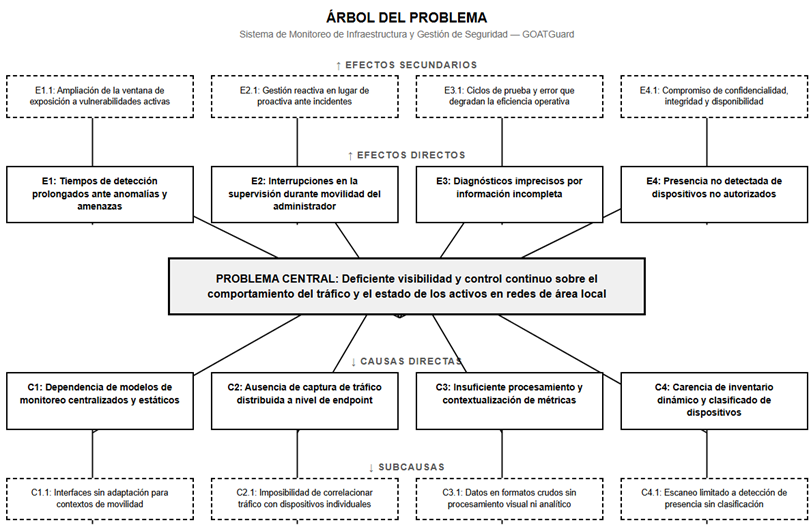
\includegraphics[width=\columnwidth]{arbol_problema.png}
\caption{Árbol de causas y efectos del problema.}
~\label{fig:arbol-problema}
\end{figure}

\subsection{Pregunta problematizadora}

\textit{¿Cómo abordar la visibilidad y control sobre el 
comportamiento del tráfico de red y el estado de los activos 
conectados en una infraestructura, considerando la necesidad de 
detectar anomalías, métricas y dispositivos de forma independiente 
de la ubicación física del administrador?}

\subsection{Justificación}

Las limitaciones descritas trascienden el plano de la comodidad 
operativa y afectan la continuidad de los servicios, la capacidad 
de respuesta del equipo responsable y la exposición a riesgos de 
seguridad interna. Cada intervalo sin supervisión amplía la ventana 
durante la cual una anomalía puede escalar hacia una afectación de 
mayor alcance, y cada diagnóstico realizado sobre información 
incompleta incrementa la probabilidad de ciclos de prueba y error 
que consumen tiempo y pueden agravar la situación original. En 
organizaciones donde la red sostiene la totalidad de los procesos 
de comunicación interna y acceso a la información, esta brecha 
representa un costo directo en términos de productividad, calidad 
del servicio y posturas de seguridad.

El abordaje del problema requiere articular conocimientos de 
distintas áreas de la ingeniería de sistemas: captura y análisis de 
tráfico desde la perspectiva de redes de datos, procesamiento y 
persistencia de volúmenes significativos de información desde la 
perspectiva de bases de datos y sistemas distribuidos, y exposición 
de resultados al administrador desde la perspectiva del desarrollo 
de software y la movilidad. La naturaleza integradora del proyecto 
justifica su desarrollo como una propuesta unificada más que como 
la mejora aislada de un componente, y habilita un escenario de 
aplicación para las competencias de infraestructura tecnológica, 
seguridad de la información e ingeniería de software establecidas 
en el marco académico del Proyecto Integrador.
\section{Objetivos}
~\label{sec:objetivos}

Los objetivos del proyecto se formulan siguiendo las fases del ciclo 
de vida del desarrollo de software, de manera que cada uno corresponde 
a una etapa específica del proceso: diseño, implementación, validación 
y despliegue. Esta correspondencia permite trazar el avance del 
proyecto frente a los hitos metodológicos adoptados.

\subsection{Objetivo general}

Desarrollar un sistema de monitoreo de tráfico de red local mediante 
el diseño, implementación e integración de sensores de captura 
distribuida, un backend de análisis centralizado y una aplicación 
móvil, con el fin de proporcionar visibilidad continua sobre el 
comportamiento del tráfico y el estado de los activos conectados a la 
red de forma independiente de la ubicación física del administrador.

\subsection{Objetivos específicos}

\begin{itemize}
    \item Diseñar la arquitectura del sistema de monitoreo, compuesta 
    por sensores de captura en endpoints, un servidor colector, un 
    motor de análisis y una aplicación móvil, mediante la definición 
    de los flujos de datos, protocolos de comunicación y estructuras 
    de almacenamiento, con el fin de establecer la base técnica sobre 
    la cual se construirán los componentes del sistema.

    \item Implementar los sensores de captura, el motor de análisis 
    con su inventario dinámico de activos y la aplicación móvil, 
    mediante la construcción e integración de cada componente según 
    la arquitectura diseñada, con el fin de recolectar el tráfico de 
    los endpoints, transformarlo en métricas contextualizadas y 
    presentarlas al administrador junto con notificaciones ante 
    comportamientos de tráfico inusuales.

    \item Validar el funcionamiento del sistema mediante la ejecución 
    de pruebas sobre los módulos de captura, análisis y visualización, 
    con el fin de verificar que los datos fluyan correctamente desde 
    los sensores hasta la aplicación móvil y que la información 
    presentada sea consistente con el tráfico real de la red.

    \item Desplegar el sistema mediante pipelines de integración y 
    entrega continua, con el fin de facilitar la publicación de la 
    aplicación móvil y la puesta en operación del backend en un 
    entorno funcional.
\end{itemize}
\section{Alcance y delimitación}
~\label{sec:alcance}

El alcance del proyecto se define sobre segmentos de red 
de pequeña o mediana escala administrados por un único 
responsable, que accede al sistema desde una aplicación móvil y cuenta 
con conocimientos técnicos en administración de redes. Los sensores de 
captura se despliegan en los endpoints bajo control del administrador, 
mientras que los dispositivos ajenos a esa gestión solo son objeto de 
detección e identificación básica a partir de técnicas de 
descubrimiento activo.

\subsection{Inclusiones}

El proyecto comprende el desarrollo de los cuatro componentes 
establecidos en el acta de constitución:

\begin{itemize}
    \item \textbf{Sensores de captura desplegables en endpoints}, 
    responsables de capturar el tráfico de red de la interfaz en la 
    que están instalados y transmitirlo hacia un servidor colector 
    centralizado dentro de la misma red local, recolectar métricas 
    básicas del estado del endpoint como uso de CPU y memoria, y 
    ejecutar descubrimiento básico de otros dispositivos presentes en 
    el segmento de red mediante técnicas como ARP.@

    \item \textbf{Backend de análisis centralizado}, encargado de 
    recibir y almacenar los datos enviados por los sensores, procesar 
    el tráfico capturado para generar métricas contextualizadas como 
    consumo de ancho de banda, retransmisiones TCP, tiempos de 
    respuesta DNS y perfiles de tráfico por dispositivo, construir y 
    mantener el inventario dinámico de activos, identificar 
    comportamientos inusuales y exponer la información procesada a 
    través de una API consumida por la aplicación móvil.

    \item \textbf{Aplicación móvil de consulta y notificación}, que 
    permite al administrador consultar el inventario de dispositivos, 
    visualizar métricas tanto a nivel de segmento de red como por 
    endpoint individual, contextualizar los dispositivos dentro del 
    segmento como representación de la topología, y recibir 
    notificaciones push ante comportamientos de tráfico inusuales.

    \item \textbf{Infraestructura de integración y entrega continua}, 
    que gestiona la compilación, pruebas automatizadas y despliegue 
    del backend, así como la publicación de la aplicación móvil.
\end{itemize}

\subsection{Exclusiones}

El proyecto no contempla los siguientes aspectos, definidos 
explícitamente como fuera de alcance:

\begin{itemize}
    \item Mecanismos de respuesta automática ante incidentes; el 
    sistema monitorea y notifica, pero no interviene sobre la red.

    \item Administración activa de la red, como denegar o permitir 
    acceso a dispositivos.

    \item Gestión o control remoto de los dispositivos conectados.

    \item Monitoreo del tráfico de dispositivos que no cuenten con 
    sensor instalado; para estos, el sistema se limita a su detección 
    e identificación básica dentro del inventario.

    \item Infraestructuras de gran escala, como redes con múltiples 
    sedes, segmentos WAN o despliegues en nubes públicas.

    \item Almacenamiento histórico ilimitado de datos de tráfico; el 
    sistema opera con ventanas de retención acotadas por la capacidad 
    de la infraestructura disponible.
\end{itemize}
\section{Marco teórico}
~\label{sec:marco-teorico}

\subsection{Modelo OSI y arquitectura TCP/IP}

El diseño y operación de sistemas de monitoreo de red se sostienen 
sobre dos modelos de referencia que describen la comunicación entre 
dispositivos de forma estratificada: el modelo OSI de siete capas 
propuesto por la Organización Internacional de Normalización 
~\cite{iso7498}, y la arquitectura TCP/IP de cuatro capas que refleja 
la implementación práctica de la suite de protocolos de Internet 
~\cite{forouzan2006transmision}. Ambos modelos abstraen la complejidad 
de las comunicaciones mediante la separación de responsabilidades: 
cada capa ofrece un servicio específico a la capa inmediatamente 
superior y se apoya en los servicios de la capa inmediatamente 
inferior, lo cual permite que los componentes de un sistema 
evolucionen de forma independiente siempre que respeten las 
interfaces entre capas~\cite{kurose2010redes}.

Las capas inferiores determinan los mecanismos sobre los cuales opera 
GOATGuard. La capa de enlace de datos (Capa 2) define la estructura 
de las tramas Ethernet~\cite{ieee8023} y las direcciones MAC, que 
permiten la identificación de dispositivos a nivel físico dentro del 
segmento local; esta capa soporta el descubrimiento de activos 
mediante el protocolo ARP~\cite{rfc826}. La capa de red (Capa 3) 
define las direcciones IP y los mecanismos de enrutamiento; sobre 
esta capa opera el protocolo ICMP~\cite{rfc792} empleado en el 
sondeo de salud del enlace hacia el proveedor de servicios. La capa 
de transporte (Capa 4) proporciona los dos protocolos que estructuran 
el transporte dual del sistema: TCP~\cite{rfc793} para la entrega 
confiable y ordenada del tráfico capturado, y UDP~\cite{rfc768} para 
la transmisión de métricas y señales de disponibilidad. Finalmente, 
la capa de aplicación (Capa 7) aloja los protocolos DNS 
~\cite{rfc1035}, HTTP~\cite{rfc9110} y los intercambios TLS 
~\cite{rfc8446} observados durante la captura, cuya inspección 
alimenta el análisis de flujos.

Aunque los dos modelos difieren en el número de capas, las funciones 
relevantes para este trabajo coinciden en ambos. Esto permite 
expresar las decisiones de diseño en términos de capas sin ambigüedad 
y asociar cada componente del sistema a una responsabilidad 
específica dentro del stack de comunicaciones~\cite{kurose2010redes}.

\subsection{Estructura de un paquete de red
}

Un paquete observado en una interfaz Ethernet sigue un esquema de 
encapsulación anidada en el que cada capa antepone sus propios 
encabezados al contenido recibido de la capa superior 
\cite{forouzan2006transmision}. En la base se encuentra el encabezado 
Ethernet de catorce bytes~\cite{ieee8023}, que incluye las 
direcciones MAC de origen y destino y el campo EtherType que indica 
el protocolo de la capa siguiente (Fig.~\ref{fig:paquete-red}). A 
continuación aparece el encabezado IP de veinte bytes en su versión 
mínima, que contiene las direcciones IP de origen y destino, el 
identificador de protocolo de transporte, el TTL y el checksum de 
cabecera. Por último se ubica el encabezado de transporte: veinte 
bytes para TCP, con números de secuencia y acuse, tamaño de ventana 
y banderas de control, u ocho bytes para UDP, con puertos y longitud 
del datagrama~\cite{stevens2004unix}.

Este conjunto de encabezados, aproximadamente cincuenta y cuatro 
bytes, concentra la totalidad de la información necesaria para 
reconstruir flujos y extraer métricas de comportamiento sin recurrir 
al contenido del payload. Las direcciones MAC identifican emisor y 
receptor dentro del segmento local; las direcciones IP, junto con 
los puertos y el protocolo de transporte, conforman la tupla de 
cinco elementos que define cada flujo de comunicación 
~\cite{kurose2010redes}; las banderas TCP permiten determinar el 
ciclo de vida de una conexión y detectar retransmisiones 
~\cite{rfc793}. El payload de aplicación, por el contrario, puede 
contener información sensible como credenciales, contenido de 
comunicaciones o datos personales, y su captura integral 
comprometería la confidencialidad de los usuarios monitoreados.
Un segundo aspecto relevante es el orden de los bytes en la 
transmisión. Los encabezados de los protocolos de red se representan 
en network byte order, que corresponde a la convención big-endian: 
el byte más significativo se transmite primero~\cite{rfc793}. Los 
sistemas operativos sobre arquitecturas x86 almacenan los datos en 
little-endian, por lo que la serialización y deserialización de 
campos numéricos requiere conversiones explícitas para garantizar la 
interoperabilidad entre emisores y receptores independientemente de 
la arquitectura subyacente~\cite{stevens2004unix}.


\begin{figure}[H]
\centering
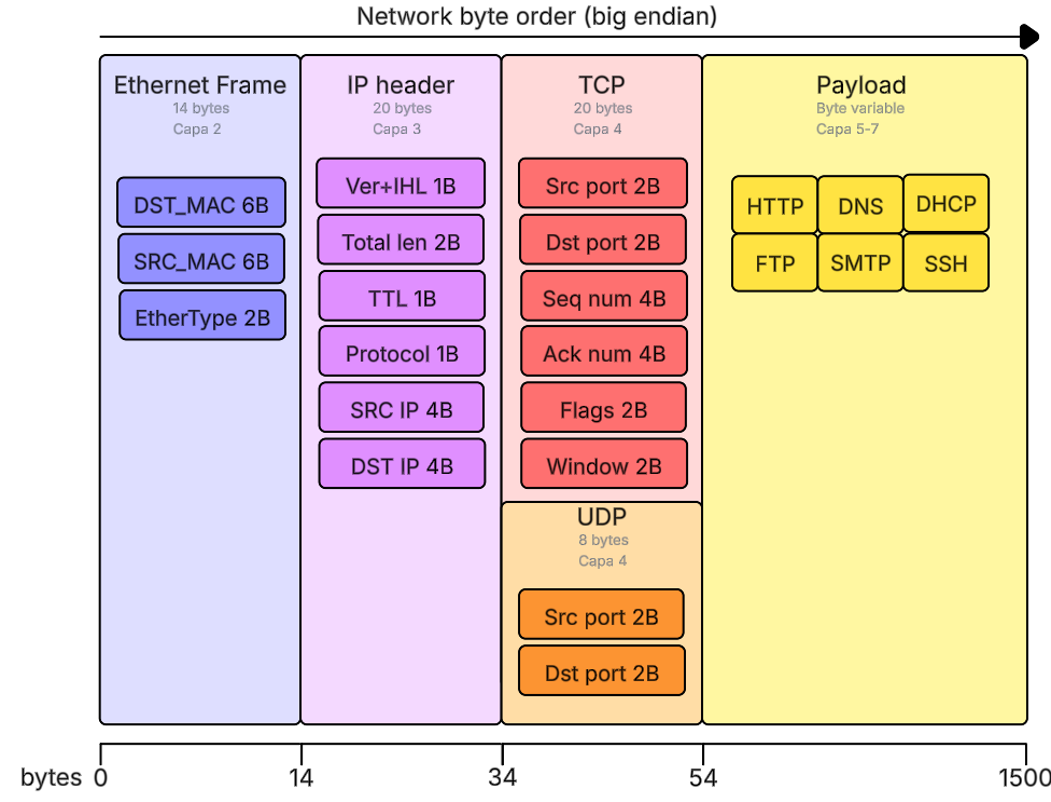
\includegraphics[width=\columnwidth]{paquete_red.png}
\caption{Estructura simplificada de un paquete de red.}
~\label{fig:paquete-red}
\end{figure}

Esta estructura justifica técnicamente la estrategia de sanitización 
adoptada por los sensores de captura: un recorte de noventa y seis 
bytes preserva los encabezados de las tres capas inferiores con 
margen para las opciones TCP, mientras que un recorte extendido a 
trescientos bytes para tráfico dirigido a los puertos asociados a 
DNS y HTTPS permite incluir el dominio consultado y la indicación de 
nombre de servidor del handshake TLS~\cite{rfc8446}, elementos con 
valor diagnóstico que no comprometen el contenido de las 
comunicaciones.

\subsection{Monitoreo de redes: captura centralizada vs distribuida}

Los enfoques tradicionales de monitoreo en redes de área local 
operan desde un único punto de observación, típicamente un servidor 
que recibe una copia del tráfico mediante un puerto mirror en el 
switch o una interfaz configurada para escuchar el segmento 
~\cite{kurose2010redes}. Sobre este modelo pasivo se articulan el 
monitoreo activo, que genera tráfico de prueba para verificar 
conectividad~\cite{forouzan2006transmision}, y herramientas de uso 
extendido como Wireshark para análisis de paquetes, Nmap para 
descubrimiento de hosts~\cite{lyon2009nmap}, Snort para detección de 
intrusos~\cite{roesch1999snort}, y plataformas empresariales como 
Zabbix o PRTG para consolidación de métricas. La limitación 
estructural de este enfoque es la pérdida de granularidad: la 
captura agregada impide atribuir un patrón anómalo al endpoint que 
lo origina, y su dependencia de consolas fijas, sumada al 
licenciamiento orientado a grandes infraestructuras, lo hace inviable 
en redes de pequeña escala.

La alternativa distribuida despliega procesos ligeros en cada 
endpoint que capturan el tráfico localmente y lo reportan a un 
servidor central~\cite{paxson1999zeek}. Esta topología preserva la 
granularidad por dispositivo y habilita la correlación directa entre 
una anomalía y su equipo responsable, a costa de instalar un 
componente en cada host y diseñar un canal de transporte que no 
sature la red ni degrade el rendimiento del endpoint. Estas 
tensiones de diseño orientan las decisiones arquitectónicas 
descritas en la Sección~\ref{sec:desarrollo}.

El modelo distribuido cuenta con un antecedente formal en la 
arquitectura IPFIX (IP Flow Information Export) especificada por la 
IETF en la RFC 5470~\cite{rfc5470}. Este documento establece un 
modelo de referencia en el que uno o varios \textit{observation 
points} dentro de un \textit{IPFIX device} alimentan un conjunto de 
\textit{metering processes} que a su vez entregan sus datos a un 
\textit{exporting process}, el cual los transmite a un 
\textit{collector} encargado de la recepción, procesamiento y 
almacenamiento (Fig.~\ref{fig:ipfix}). La correspondencia con 
GOATGuard es directa: los sensores de captura cumplen el rol de 
observation point y metering process sobre cada endpoint, mientras 
que el backend actúa como collector que consolida, procesa y 
persiste los datos reportados. Esta correspondencia no implica 
adoptar el protocolo IPFIX como tal sino reconocer que la 
descomposición funcional del sistema se apoya en un modelo de 
referencia ya estandarizado.

\begin{figure}[H]
\centering
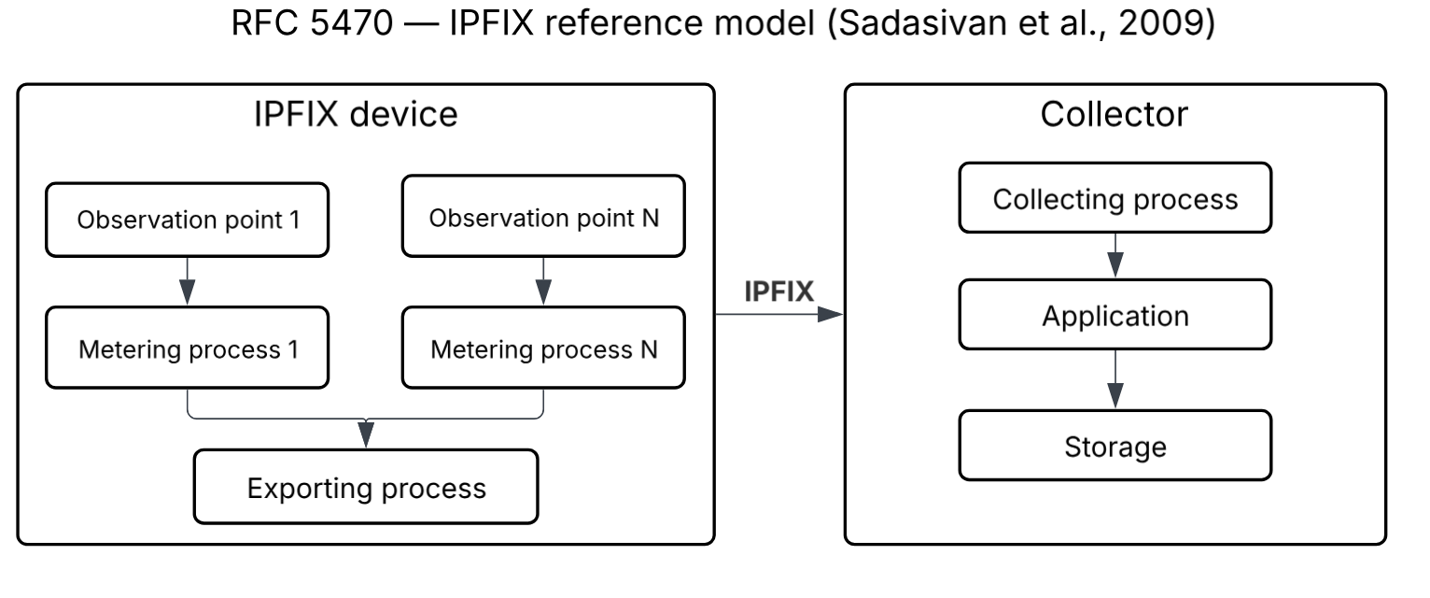
\includegraphics[width=\columnwidth]{ipfix_rfc5470.png}
\caption{Modelo de referencia IPFIX definido en la RFC 5470~\cite{rfc5470}. La arquitectura de GOATGuard mapea sus sensores al rol de observation point y metering process, y el backend al rol de collector.}
~\label{fig:ipfix}
\end{figure}

\subsection{Descubrimiento y clasificación de activos}

El descubrimiento de dispositivos parte del escaneo activo: 
solicitudes ARP~\cite{rfc826} para resolver direcciones IP y MAC 
dentro del segmento de enlace, sondeos ICMP~\cite{rfc792} para 
confirmar alcanzabilidad, y pruebas a puertos TCP/UDP específicos 
para revelar servicios expuestos; herramientas como Nmap combinan 
estas técnicas en un inventario inicial~\cite{lyon2009nmap}. Dos 
limitaciones acotan este enfoque. Primero, la información recolectada 
se reduce a presencia y datos técnicos básicos, sin distinguir entre 
una estación de trabajo, una impresora, un dispositivo IoT o un 
equipo personal no autorizado. Segundo, los escaneos se ejecutan de 
forma periódica y no continua, dejando ventanas durante las cuales 
un dispositivo puede conectarse sin ser detectado hasta el siguiente 
ciclo.

La técnica de network fingerprinting responde parcialmente a la 
primera limitación combinando señales de múltiples capas del stack 
~\cite{lippmann2003fingerprint}: el prefijo OUI de la MAC identifica 
al fabricante, los puertos abiertos y banners de servicios revelan 
el sistema operativo y las aplicaciones, y el patrón de 
comunicación, como la frecuencia de consultas DNS o los destinos 
recurrentes, permite inferir el rol operativo del dispositivo. La 
combinación de estos indicadores habilita la transición desde un 
listado plano hacia un inventario clasificado. El sistema propuesto 
integra el descubrimiento ARP ejecutado por los sensores con el 
registro explícito de los endpoints instrumentados, manteniendo 
trazabilidad tanto de los dispositivos bajo control directo como de 
los observados pasivamente en el segmento.

\subsection{Detección de anomalías por métodos estadísticos adaptativos}

La detección de anomalías en series temporales consiste en 
identificar observaciones que se desvían significativamente del 
comportamiento esperado dado el historial previo de la misma 
variable~\cite{chandola2009anomaly}. En el contexto del monitoreo 
de infraestructura, cada métrica asociada a un dispositivo produce 
una secuencia de valores en el tiempo cuya distribución no es 
conocida a priori y varía entre dispositivos: una estación de 
desarrollo puede presentar un consumo de CPU sostenido del sesenta 
por ciento durante compilaciones, mientras que un servidor de 
archivos puede operar establemente por debajo del diez por ciento. 
Un método de detección útil debe construir un perfil individual 
para cada dispositivo y métrica, adaptarse a cambios legítimos en 
el comportamiento, y operar en línea sin requerir un conjunto de 
entrenamiento previo~\cite{chandola2009anomaly}.

Los umbrales fijos constituyen el enfoque más simple pero resultan 
inadecuados para esta tarea: un límite absoluto definido globalmente 
ignora el perfil particular de cada dispositivo y produce falsos 
positivos en los que operan legítimamente cerca del umbral, al 
tiempo que pierde anomalías relativas en dispositivos con líneas 
base bajas~\cite{montgomery2013spc}. El cálculo de Z-Score sobre la 
media aritmética acumulada corrige parcialmente este problema al 
normalizar por la desviación típica observada, pero la media 
acumulada pondera por igual todas las observaciones históricas y 
tarda horas en converger cuando el comportamiento del dispositivo 
cambia de forma sostenida, lo que genera falsas alarmas durante el 
periodo de adaptación.

La media móvil ponderada exponencialmente (Exponentially Weighted 
Moving Average, EWMA) propuesta originalmente por Roberts 
~\cite{roberts1959ewma} y consolidada como herramienta de control 
estadístico por Hunter~\cite{hunter1986ewma} resuelve este problema 
asignando pesos que decrecen geométricamente con la antigüedad de 
cada observación. Lucas y Saccucci~\cite{lucas1990ewma} ampliaron 
posteriormente este esquema con el análisis de sus propiedades de 
detección y con extensiones para señales con varianza variable. El 
baseline se actualiza en cada ciclo mediante la recurrencia
\begin{equation}
\mu_t = \alpha \cdot x_t + (1-\alpha) \cdot \mu_{t-1},
\label{eq:ewma}
\end{equation}
donde $\mu_t$ es el baseline estimado en el ciclo $t$, $x_t$ la 
observación actual, y $\alpha \in (0,1)$ el factor de suavizado que 
determina la velocidad de adaptación del estimador. Un valor de 
$\alpha$ cercano a uno produce un baseline altamente reactivo al 
último dato, mientras que un valor cercano a cero produce un 
baseline estable pero lento para adaptarse a cambios reales. El 
peso que una observación retiene tras $k$ ciclos es 
$\alpha \cdot (1-\alpha)^k$, lo que define una memoria efectiva 
finita a partir de la cual los datos antiguos se consideran 
olvidados~\cite{lucas1990ewma}.

La varianza se estima con el mismo principio exponencial 
(Exponentially Weighted Moving Variance, EWMV) mediante
\begin{equation}
{\sigma^2_t = (1-\alpha) \cdot \left[\sigma^2_{t-1} + \alpha \cdot (x_t - \mu_{t-1})^2\right],}
\label{eq:ewmv}
\end{equation}
donde $(x_t - \mu_{t-1})^2$ cuantifica la discrepancia entre la 
observación actual y el baseline anterior. Con el baseline y la 
varianza adaptativos, el Z-Score se calcula como
\begin{equation}
Z_t = \frac{x_t - \mu_{t-1}}{\sqrt{\sigma^2_{t-1}}},
\label{eq:zscore}
\end{equation}
contra el baseline y varianza del ciclo anterior, antes de 
actualizarlos con la observación actual. Este orden preserva la 
sensibilidad del estimador ante anomalías: si los estadísticos se 
actualizaran primero, la anomalía se absorbería parcialmente en el 
baseline antes de ser evaluada~\cite{montgomery2013spc}.

Bajo el supuesto de distribución aproximadamente normal en 
condiciones de operación estable, el Z-Score admite una 
interpretación probabilística directa. La probabilidad de que una 
observación produzca $|Z|>2$ bajo ese supuesto es 4.56\%, y la de 
que supere $|Z|>3$ es 0.27\%, lo que permite asignar una medida de 
rareza estadística a cada evaluación y establecer umbrales de 
severidad con significado probabilístico explícito 
~\cite{montgomery2013spc}.

\subsection{Arquitecturas cliente-servidor y patrones de integración}

La exposición de los datos procesados hacia la aplicación móvil se 
apoya en el estilo arquitectónico REST (Representational State 
Transfer) formulado por Fielding~\cite{fielding2000rest}. REST 
establece un conjunto de restricciones para sistemas distribuidos 
basados en HTTP, entre las cuales destacan la separación entre 
cliente y servidor, la ausencia de estado de sesión en el servidor, 
la identificación de recursos mediante URIs y la manipulación de 
esos recursos a través de los métodos estándar del protocolo HTTP 
~\cite{rfc9110}. La restricción \textit{stateless} implica que cada 
petición del cliente contiene toda la información necesaria para 
ser procesada, lo cual simplifica la escalabilidad horizontal del 
servidor pero requiere un mecanismo alternativo para mantener la 
autenticación del usuario entre peticiones, función que típicamente 
cumplen los tokens JWT~\cite{rfc7519} adjuntados en cada petición.

El modelo de petición y respuesta de HTTP es eficaz para consultas 
puntuales, pero presenta limitaciones en escenarios de monitoreo 
continuo donde el estado del sistema evoluciona de forma constante 
y el cliente necesita reflejar esos cambios sin retrasos 
significativos. El polling periódico, en el que el cliente repite 
una petición cada cierto intervalo, introduce sobrecarga de 
encabezados HTTP redundantes, consumo innecesario de ancho de banda 
y latencia variable entre la generación de un dato en el servidor y 
su visualización en el cliente~\cite{rfc9110}. El protocolo 
WebSocket~\cite{rfc6455} atiende este escenario mediante un canal 
bidireccional persistente establecido sobre una única conexión TCP 
tras un handshake inicial de actualización desde HTTP;@una vez 
abierto, tanto servidor como cliente pueden enviar mensajes en 
cualquier momento sin la sobrecarga de encabezados de HTTP, lo que 
habilita la notificación inmediata de eventos como alertas o 
actualizaciones de estado.

En sistemas compuestos por múltiples procesos que deben compartir 
información, el patrón \textit{Shared Database} descrito por Hohpe 
y Woolf~\cite{hohpe2003eip} propone una base de datos común como 
punto de acoplamiento entre procesos independientes. Cada proceso 
opera sobre su propio ciclo de vida, con sus propios recursos y 
perfil de carga, y accede a la base de datos para leer los datos 
que otros procesos produjeron o para escribir los suyos. Este 
patrón resulta apropiado cuando los procesos tienen perfiles de 
ejecución heterogéneos, ya que el aislamiento a nivel de proceso 
del sistema operativo garantiza que un fallo en uno de ellos no 
afecta la operación de los demás~\cite{silberschatz2018os}, a 
diferencia de una arquitectura monolítica en la que todas las 
responsabilidades comparten el mismo espacio de ejecución.

La organización interna de cada proceso se apoya en patrones de 
diseño clásicos documentados por Gamma et al.~\cite{gof1994}. Los 
patrones relevantes para este trabajo incluyen Strategy, que 
desacopla un algoritmo de su contexto de uso mediante una interfaz 
común; Mediator, que centraliza la comunicación entre componentes 
en un orquestador que conoce a todos los participantes y evita el 
acoplamiento directo entre ellos; y la inversión de control 
implementada mediante callbacks, que permite a un módulo invocar 
comportamiento definido externamente sin conocer los detalles de 
implementación~\cite{gof1994}. A estos se suman patrones 
específicos de sistemas concurrentes documentados por Schmidt et 
al.~\cite{schmidt2000posa2}, como Thread-per-Client, en el cual 
cada conexión entrante se atiende en un hilo dedicado para aislar 
los fallos individuales; y el patrón Productor-Consumidor descrito 
por Buschmann et al.~\cite{buschmann1996posa}, que coordina la 
transferencia de datos entre dos hilos con velocidades distintas 
mediante un buffer compartido protegido por exclusión mutua. La 
aplicación concreta de estos patrones se describe en la Sección 
~\ref{sec:desarrollo}.
\section{Marco legal y normativo}
\label{sec:marco-legal}

La operación de un sistema que captura tráfico de red y registra 
información sobre los dispositivos conectados debe ajustarse al marco 
legal aplicable a la protección de los datos personales y al acceso 
a sistemas informáticos. Este ajuste se evalúa tradicionalmente desde 
los tres pilares de la seguridad de la información, conocidos como 
tríada CIA: confidencialidad, que exige que la información solo sea 
accesible a quienes tienen autorización explícita; integridad, que 
exige que los datos no sean alterados de forma indebida durante su 
tratamiento; y disponibilidad, que exige que la información se 
mantenga accesible para los usuarios legítimos en el momento en que 
la requieran. Las decisiones de diseño descritas en la Sección 
\ref{sec:desarrollo}, como la sanitización de payload, la 
autenticación basada en tokens firmados, el cifrado en tránsito y la 
separación de procesos para aislar fallos, responden de forma directa 
a estos tres pilares.

En el ordenamiento jurídico colombiano, las normas aplicables a 
GOATGuard se concentran en tres bloques: la tipificación de los 
delitos contra la confidencialidad, integridad y disponibilidad de 
los datos y los sistemas informáticos \cite{ley1273_2009}; el régimen 
general de protección de datos personales \cite{ley1581_2012} y su 
decreto reglamentario parcial \cite{decreto1377_2013}; y las 
disposiciones sobre monitoreo laboral \cite{ley2466_2025}. La 
Tabla~\ref{tab:marco-legal} sintetiza los artículos relevantes y la 
forma en que el diseño del sistema responde a cada uno de ellos.

\begin{table*}[!t]
\centering
\caption{Normativa colombiana aplicable al sistema y su impacto en el diseño.}
\label{tab:marco-legal}
\begin{tabular}{@{}p{2.5cm}p{1.8cm}p{5cm}p{6cm}@{}}
\toprule
\textbf{Norma} & \textbf{Artículo} & \textbf{Materia regulada} & \textbf{Respuesta de diseño en GOATGuard} \\
\midrule
Ley 1273 de 2009 & 269A & Acceso abusivo a sistema informático & La instalación del sensor requiere autorización expresa del responsable de la red. \\[4pt]
Ley 1273 de 2009 & 269C & Interceptación de datos informáticos & La captura de paquetes se realiza bajo autorización documentada; el payload se sanitiza para no interceptar contenido de comunicaciones. \\[4pt]
Ley 1581 de 2012 & 4 (libertad) & Consentimiento del titular de los datos & Los usuarios de los endpoints son informados del monitoreo antes de la puesta en operación. \\[4pt]
Ley 1581 de 2012 & 4 (finalidad) & Tratamiento únicamente para el fin declarado & Los datos capturados se usan solo para la detección de anomalías y el inventario de activos, no para otros propósitos. \\[4pt]
Ley 1581 de 2012 & 6 & Excepción para fines académicos o de investigación & Aplicable al presente proyecto, siempre que se mantenga la anonimización del contenido. \\[4pt]
Decreto 1377 de 2013 & 3 & Aviso previo de privacidad & El despliegue del sistema incluye la entrega de un aviso de privacidad a los usuarios antes de iniciar la captura. \\[4pt]
Ley 2466 de 2025 & N/A & Monitoreo en el ámbito laboral & En escenarios empresariales, la operación del sistema requiere el consentimiento explícito y documentado del trabajador. \\
\bottomrule
\end{tabular}
\end{table*}

Tres decisiones concretas del diseño resultan del cruce con la 
tabla anterior. La primera es la sanitización del payload en el 
sensor de captura: el recorte dinámico de los paquetes preserva los 
encabezados necesarios para el análisis de flujos pero elimina el 
contenido de las comunicaciones, lo que reduce el alcance de la 
captura al estrictamente necesario para el fin declarado y elimina la 
exposición a contenido sensible que podría constituir una 
interceptación indebida en el sentido del artículo 269C. La segunda 
es el control de acceso al sistema mediante autenticación con 
contraseña hasheada y emisión de tokens JWT con expiración definida, 
que limita el acceso a los datos procesados únicamente al 
administrador autorizado, en concordancia con el principio de 
confidencialidad. La tercera es la generación de un registro 
persistente de las operaciones realizadas por el pipeline y la API, 
que permite auditar el uso del sistema y respaldar la trazabilidad 
exigida por el régimen general de protección de datos.

La aplicación académica del sistema se encuadra dentro de la 
excepción científica del artículo 6 de la Ley 1581 de 2012, 
condicionada a la anonimización del tratamiento. El equipo adopta 
esta condición como criterio operativo: ningún identificador de 
usuario individual se persiste en el sistema, y los identificadores 
de dispositivos se construyen a partir de atributos técnicos 
(hostname y dirección MAC) que no permiten por sí mismos vincular la 
actividad observada con una persona natural específica. La extensión 
del sistema a entornos productivos, donde esta excepción no aplicaría 
de forma automática, requeriría la gestión explícita de los 
consentimientos correspondientes según la Ley 2466 de 2025 en 
contextos laborales.

La totalidad de las actividades de captura, procesamiento y pruebas 
ejecutadas durante el desarrollo del proyecto se circunscriben a 
entornos controlados dispuestos por el equipo de investigación, 
conformados por redes locales de uso académico y por los endpoints 
propios de los integrantes del proyecto. Los datos capturados durante 
estas pruebas no se transfieren a terceros, no se integran a 
sistemas en producción y no se emplean para ningún fin ajeno al de 
la validación técnica del prototipo. La eventual adopción del sistema 
en un entorno productivo o empresarial queda por fuera del alcance 
del presente trabajo y requeriría, como condición previa, la 
formalización de los consentimientos, autorizaciones y controles 
adicionales que el marco normativo señalado exige para el tratamiento 
de datos personales fuera de la excepción científica.
\section{Metodología}
\label{sec:metodologia}

El desarrollo del proyecto adopta una metodología basada en la 
adaptación del Proceso Unificado Racional (Rational Unified Process, 
RUP) al contexto del Proyecto Integrador, complementada con 
prácticas iterativas e incrementales propias del desarrollo ágil 
moderno. La elección responde a tres características del proyecto: 
la duración semestral con entregables formales por fase, que se 
alinea con el ciclo de vida definido por hitos del RUP; la naturaleza 
iterativa del desarrollo, que requiere ciclos cortos de construcción 
y validación dentro de cada fase; y la necesidad de gestión explícita 
de riesgos técnicos, particularmente en componentes sensibles como la 
captura de tráfico a bajo nivel y el pipeline de análisis distribuido 
\cite{kruchten2003rup}.

\subsection{Adaptación de RUP al Proyecto Integrador}

El RUP organiza el ciclo de vida del software en cuatro fases 
secuenciales que separan el tipo de trabajo predominante en cada 
momento: Inicio, Elaboración, Construcción y Transición 
\cite{jacobson1999up}. Cada fase se desarrolla de forma iterativa 
mediante ciclos numerados 1 a $k$, donde el número de iteraciones 
depende de la complejidad del trabajo específico de la fase. La 
adaptación al Proyecto Integrador conserva las cuatro fases del 
modelo original y les asocia una etapa del proyecto, un conjunto de 
artefactos de cierre y mecanismos de retroalimentación entre fases. 
El esquema resultante se ilustra en la Fig.~\ref{fig:diagrama-rup}.

\begin{figure}[H]
\centering
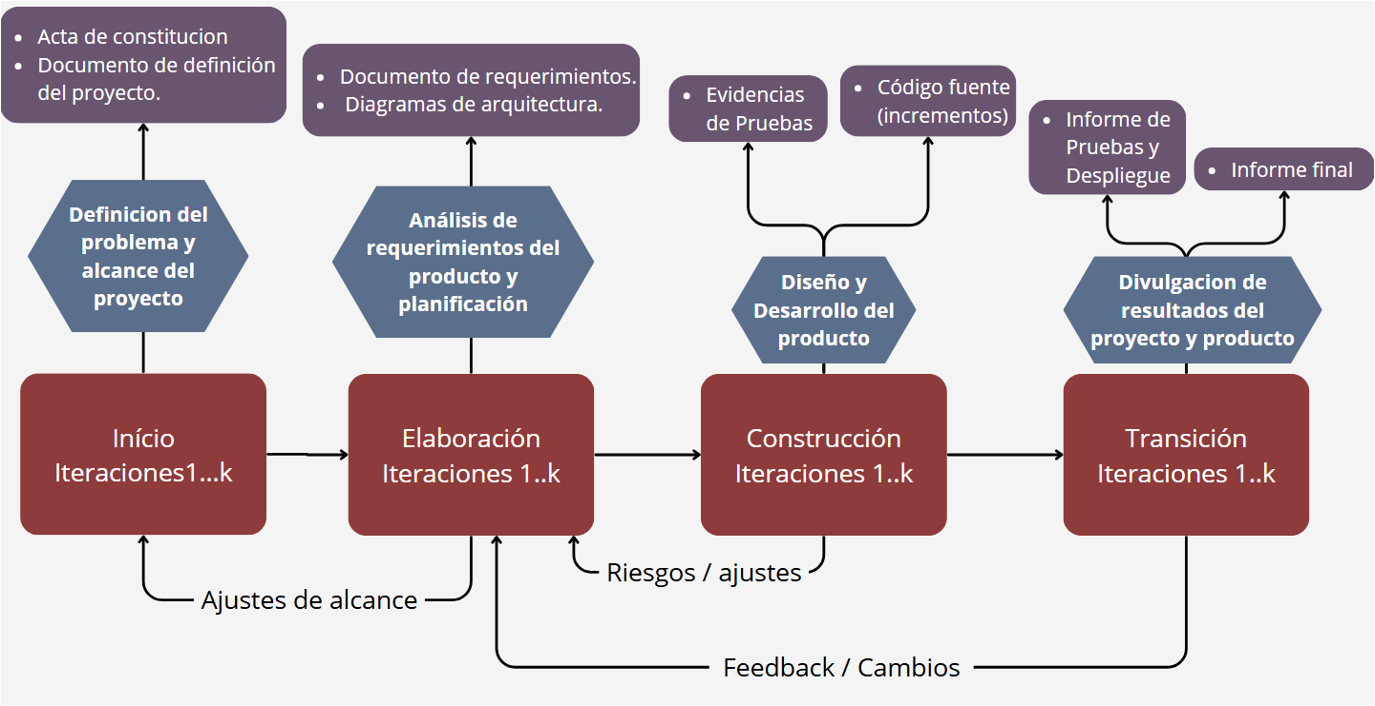
\includegraphics[width=\columnwidth]{diagrama_rup.png}
\caption{Adaptación de las cuatro fases del RUP al ciclo de vida del Proyecto Integrador, con sus respectivas etapas, artefactos de cierre y retroalimentaciones entre fases.}
\label{fig:diagrama-rup}
\end{figure}

La fase de Inicio corresponde a la etapa de definición del problema y 
alcance del proyecto, y produce como artefactos de cierre el acta de 
constitución y el documento de definición. La fase de Elaboración 
corresponde a la etapa de análisis de requerimientos y planificación, 
y cierra con el documento de requerimientos y los diagramas de 
arquitectura. La fase de Construcción corresponde a la etapa de 
diseño y desarrollo del producto, y produce las evidencias de pruebas 
y el código fuente de los incrementos. La fase de Transición 
corresponde a la etapa de divulgación de resultados del proyecto y 
del producto, y produce el informe de pruebas y despliegue junto con 
el informe final.

Entre fases operan tres flujos de retroalimentación. Los ajustes de 
alcance originados en Elaboración pueden afectar los supuestos 
establecidos durante Inicio. Los riesgos y ajustes surgidos durante 
Construcción retroalimentan las decisiones de Elaboración. Los 
hallazgos del proceso de retroalimentación y los cambios identificados 
en etapas finales se reinyectan hacia fases tempranas, garantizando 
que los artefactos producidos al cierre de cada hito reflejen el 
estado real del desarrollo y no una especificación congelada al 
inicio del proyecto.

\subsection{Fases, hitos y artefactos}

La fase de \textit{Inicio} establece el caso de negocio y delimita el 
sistema mediante la identificación del problema, las causas que lo 
originan y los actores involucrados. Los artefactos producidos son el 
acta de constitución del proyecto, que fija el alcance y las 
exclusiones, y el documento de definición, que desarrolla el árbol 
del problema, los objetivos y la primera revisión del estado del arte 
que justifica la viabilidad técnica del enfoque propuesto.

La fase de \textit{Elaboración} traduce los objetivos en 
requerimientos verificables y establece la estructura técnica del 
sistema. Los requerimientos funcionales y no funcionales se 
documentan siguiendo el estándar IEEE 830, con identificadores 
únicos, prioridades y criterios de aceptación que habilitan la 
trazabilidad posterior hacia los casos de prueba. En paralelo se 
construyen los diagramas de arquitectura C4 (contexto, contenedores, 
componentes) que describen la descomposición del sistema y las 
interfaces entre componentes, junto con la matriz de riesgos que 
califica cada riesgo identificado en términos de probabilidad e 
impacto.

La fase de \textit{Construcción} es la más extensa del ciclo y se 
ejecuta de forma iterativa. Cada ciclo produce un incremento 
funcional del sistema: primero el núcleo del sensor de captura con 
su canal TCP y el receptor correspondiente; luego el canal UDP de 
métricas y el motor de persistencia en PostgreSQL; después el 
pipeline de análisis con Zeek y el motor de detección de anomalías; 
posteriormente la API REST, el canal WebSocket y la aplicación móvil; 
y finalmente la configuración de la infraestructura de integración y 
entrega continua. Cada iteración se cierra con pruebas unitarias e 
integración del incremento producido, que en conjunto conforman las 
evidencias de prueba y el código fuente versionado de los 
incrementos.

La fase de \textit{Transición} evalúa el éxito del proyecto mediante 
la comparación directa con los objetivos establecidos: revisión de 
los entregables, contrastación entre funcionalidades implementadas y 
requerimientos especificados, validación de las pruebas realizadas y 
medición del cumplimiento del cronograma. El resultado se consolida 
en el informe de pruebas y despliegue, y culmina con la producción 
del informe de investigación y su sustentación ante 
la Jornada de Socialización de Proyectos Integradores de la Facultad 
de Ingeniería de Sistemas e Informática de la Universidad Pontificia 
Bolivariana.

\subsection{Herramientas de gestión, control de versiones e integración continua}

Las fases descritas en las secciones anteriores requieren un sustrato
operativo que preserve la trazabilidad de cada decisión, mantenga el
estado compartido del código entre los integrantes del equipo y provea
retroalimentación automatizada sobre la calidad de cada incremento.
Este sustrato se articula mediante un sistema de control de versiones
distribuido, una plataforma de gestión del trabajo alineada con los
requerimientos funcionales, y un conjunto de pipelines de integración
y entrega continua que ejecutan sobre cada cambio las verificaciones
necesarias antes de aceptarlo como parte del producto en
construcción.

\subsubsection{Control de versiones y gestión del trabajo}

El sistema se mantiene en dos repositorios Git alojados en GitHub,
uno para el backend (\texttt{goatguard-server}) y otro para la
aplicación móvil (\texttt{goatguard-app}). La separación responde a
la divergencia de ciclos de vida, entornos de ejecución y
dependencias tecnológicas de ambos componentes: el backend evoluciona
en Python sobre contenedores Linux mientras que la aplicación móvil
lo hace en Dart sobre empaquetamiento Android. Mantenerlos en
repositorios distintos permite que cada uno progrese de forma
independiente y habilita pipelines de validación especializados para
cada stack. El código del agente de captura, por compartir el
runtime Python con el backend y por su naturaleza auxiliar respecto
al colector, se conserva dentro del repositorio del servidor para
preservar la coherencia del canal binario descrito en la
Sección~\ref{subsec:sensor}.

La estrategia de ramas adoptada es de tipo \textit{trunk-based}:
existe una única rama principal \texttt{main} que representa en todo
momento el estado aceptado del sistema, y los cambios se integran
mediante \textit{pull requests} sujetos a revisión cruzada entre los
tres integrantes del equipo antes de ser fusionados. Esta política,
acordada como práctica del equipo más que impuesta por reglas
automatizadas del repositorio, cumple la función de auditoría técnica
previa al merge y distribuye el conocimiento del código entre los
desarrolladores, evitando la concentración del criterio sobre zonas
específicas del sistema.

La planificación de las iteraciones de Construcción se coordina
mediante un tablero Jira, en el que los requerimientos funcionales
se descomponen en historias y tareas con trazabilidad hacia los
identificadores RF correspondientes. Jira complementa al histórico
de Git: este último registra la evolución del código, mientras que
aquel conserva el razonamiento de alto nivel y el avance por
iteración.

\subsubsection{Integración y entrega continua como práctica
metodológica}

Los pipelines de integración y entrega continua no constituyen un
aspecto meramente operativo del proyecto sino una pieza metodológica
central, en el sentido planteado por Humble y
Farley~\cite{humble2010cd}: cada cambio sobre la rama principal
debe atravesar un conjunto de verificaciones automáticas en una
ventana acotada de tiempo, de modo que el costo de detectar una
regresión se mantenga proporcional a la magnitud del cambio que la
introdujo y no se acumule hasta el final de la iteración. En el
contexto del RUP adoptado por el proyecto~\cite{kruchten2003rup},
esta práctica materializa el mecanismo de retroalimentación entre
Construcción y Elaboración: cuando una prueba automatizada contradice
un supuesto consignado en la fase de Elaboración, la evidencia queda
registrada en el mismo commit que introduce el cambio, y el
artefacto correspondiente puede revisarse antes del siguiente hito.

La Tabla~\ref{tab:gestion-rup} sintetiza la correspondencia entre
las cuatro fases del RUP adaptado, los artefactos de gestión que
produce cada una y las herramientas concretas empleadas para
materializarlos. La descripción técnica detallada de los pipelines,
las suites de pruebas y los artefactos de despliegue se desarrolla
en la Sección~\ref{subsec:cicd}.

\begin{table}[ht]
\centering
\caption{Correspondencia entre fases del RUP adaptado, artefactos de gestión y herramientas.}
\label{tab:gestion-rup}
\footnotesize
\begin{tabular}{@{}p{1.8cm}p{2.8cm}p{2.5cm}@{}}
\toprule
\textbf{Fase} & \textbf{Artefacto de gestión} & \textbf{Herramienta} \\
\midrule
Inicio & Acta de constitución, definición del problema & Documentos versionados en repositorio \\[3pt]
Elaboración & Backlog priorizado, diagramas de arquitectura & Jira, repositorios Git \\[3pt]
Construcción & Commits, pull requests, artefactos de CI & GitHub, GitHub Actions \\[3pt]
Transición & Imágenes OCI, APK, informe final & GHCR, artefactos de GitHub Actions \\
\bottomrule
\end{tabular}
\end{table}
\section{Diseño y desarrollo del producto}
~\label{sec:desarrollo}

La presente sección describe el diseño y la implementación del sistema 
a partir de los requerimientos especificados, la arquitectura base 
definida durante la fase de Elaboración, y las decisiones técnicas 
adoptadas durante la fase de Construcción. La organización del 
contenido sigue la descomposición natural del sistema: primero el 
análisis de requerimientos (Sección~\ref{subsec:requerimientos}), 
luego el diseño arquitectónico global (Sección 
~\ref{subsec:arquitectura}), y a continuación la implementación de 
cada componente en el orden en que se integran durante el ciclo de 
vida del dato: el sensor de captura (Sección~\ref{subsec:sensor}), el 
backend y su pipeline de análisis (Sección~\ref{subsec:backend}), el 
motor de detección de anomalías (Sección~\ref{subsec:motor}), la capa 
de exposición mediante API REST y WebSocket (Sección 
~\ref{subsec:api}), y la infraestructura de integración y entrega 
continua (Sección~\ref{subsec:cicd}).

\subsection{Análisis y especificación de requerimientos}
~\label{subsec:requerimientos}

La especificación de requerimientos del sistema se documentó 
siguiendo el estándar IEEE 830, con identificadores únicos, 
prioridad de desarrollo, entradas y salidas, precondiciones, 
postcondiciones y flujos básico y alternativo para cada requerimiento 
funcional. El trabajo produjo 54 requerimientos funcionales (RF-01 a 
RF-54) distribuidos en los cuatro módulos del sistema, y seis 
categorías de requerimientos no funcionales que abarcan rendimiento, 
seguridad, fiabilidad, disponibilidad, mantenibilidad y portabilidad.

La Tabla~\ref{tab:rf-resumen} presenta la distribución de 
requerimientos por módulo junto con una síntesis de las 
responsabilidades cubiertas. La agrupación coincide con la 
descomposición arquitectónica descrita en la Sección 
~\ref{subsec:arquitectura} y permite trazar cada módulo a su conjunto 
de requerimientos asociados.

\begin{table}[ht]
\centering
\caption{Distribución de requerimientos funcionales por módulo del sistema.}
~\label{tab:rf-resumen}
\begin{tabular}{@{}p{2.3cm}cp{4cm}@{}}
\toprule
\textbf{Módulo} & \textbf{RF} & \textbf{Responsabilidades cubiertas} \\
\midrule
Sensor de captura & RF-01 a RF-05 & Captura de tráfico, métricas del endpoint, descubrimiento ARP, registro y consentimiento. \\[4pt]
Backend y pipeline & RF-06 a RF-25 & Recepción y persistencia, análisis de flujos, cálculo de métricas contextualizadas, inventario de activos. \\[4pt]
Motor de anomalías & RF-26 a RF-35 & Baselines por dispositivo, detección EWMA, filtro de persistencia, generación de alertas. \\[4pt]
API y WebSocket & RF-36 a RF-45 & Autenticación, endpoints de consulta, canal de eventos en tiempo real, notificaciones. \\[4pt]
Aplicación móvil & RF-46 a RF-54 & Login, dashboard, inventario, detalle de dispositivo, alertas, notificaciones push. \\
\bottomrule
\end{tabular}
\end{table}

Los requerimientos se priorizaron en tres niveles: \textit{Alta} para 
aquellos cuya ausencia impide la operación básica del sistema, 
\textit{Media} para los que amplían la utilidad sin ser 
bloqueantes, y \textit{Baja} para los que representan mejoras 
incrementales. Esta priorización orientó el orden de las iteraciones 
de Construcción y permitió organizar la batería de pruebas para 
cubrir primero las rutas críticas del sistema.

\subsection{Diseño arquitectónico}
~\label{subsec:arquitectura}

La arquitectura del sistema se describe en tres niveles de 
abstracción, siguiendo el modelo C4 de Simon Brown: contenedores, 
componentes y despliegue. El nivel de contexto (actores externos) se 
aborda implícitamente en la Sección~\ref{sec:alcance}, donde se 
caracterizaron el administrador como único actor humano y los 
endpoints como elementos de entrada al sistema.

\subsubsection{Vista de contenedores y componentes}

El sistema se descompone en tres subsistemas principales que se 
comunican mediante canales bien definidos. El primero es el sensor 
de captura, desplegado en cada endpoint monitoreado, que expone dos 
interfaces hacia el backend: \texttt{IEndpointMetrics} para el envío 
periódico de métricas del sistema operativo por UDP, e 
\texttt{IPcapStream} para la transmisión continua de paquetes 
sanitizados por TCP.@ El segundo es el backend centralizado, que 
internamente se divide en cinco subsistemas de propósito específico 
conectados mediante interfaces internas. El tercero es la aplicación 
móvil, que consume las interfaces públicas del backend 
(\texttt{IRestApi} e \texttt{IWebSocket}) para presentar información 
al administrador.

\begin{figure}[H]
\centering
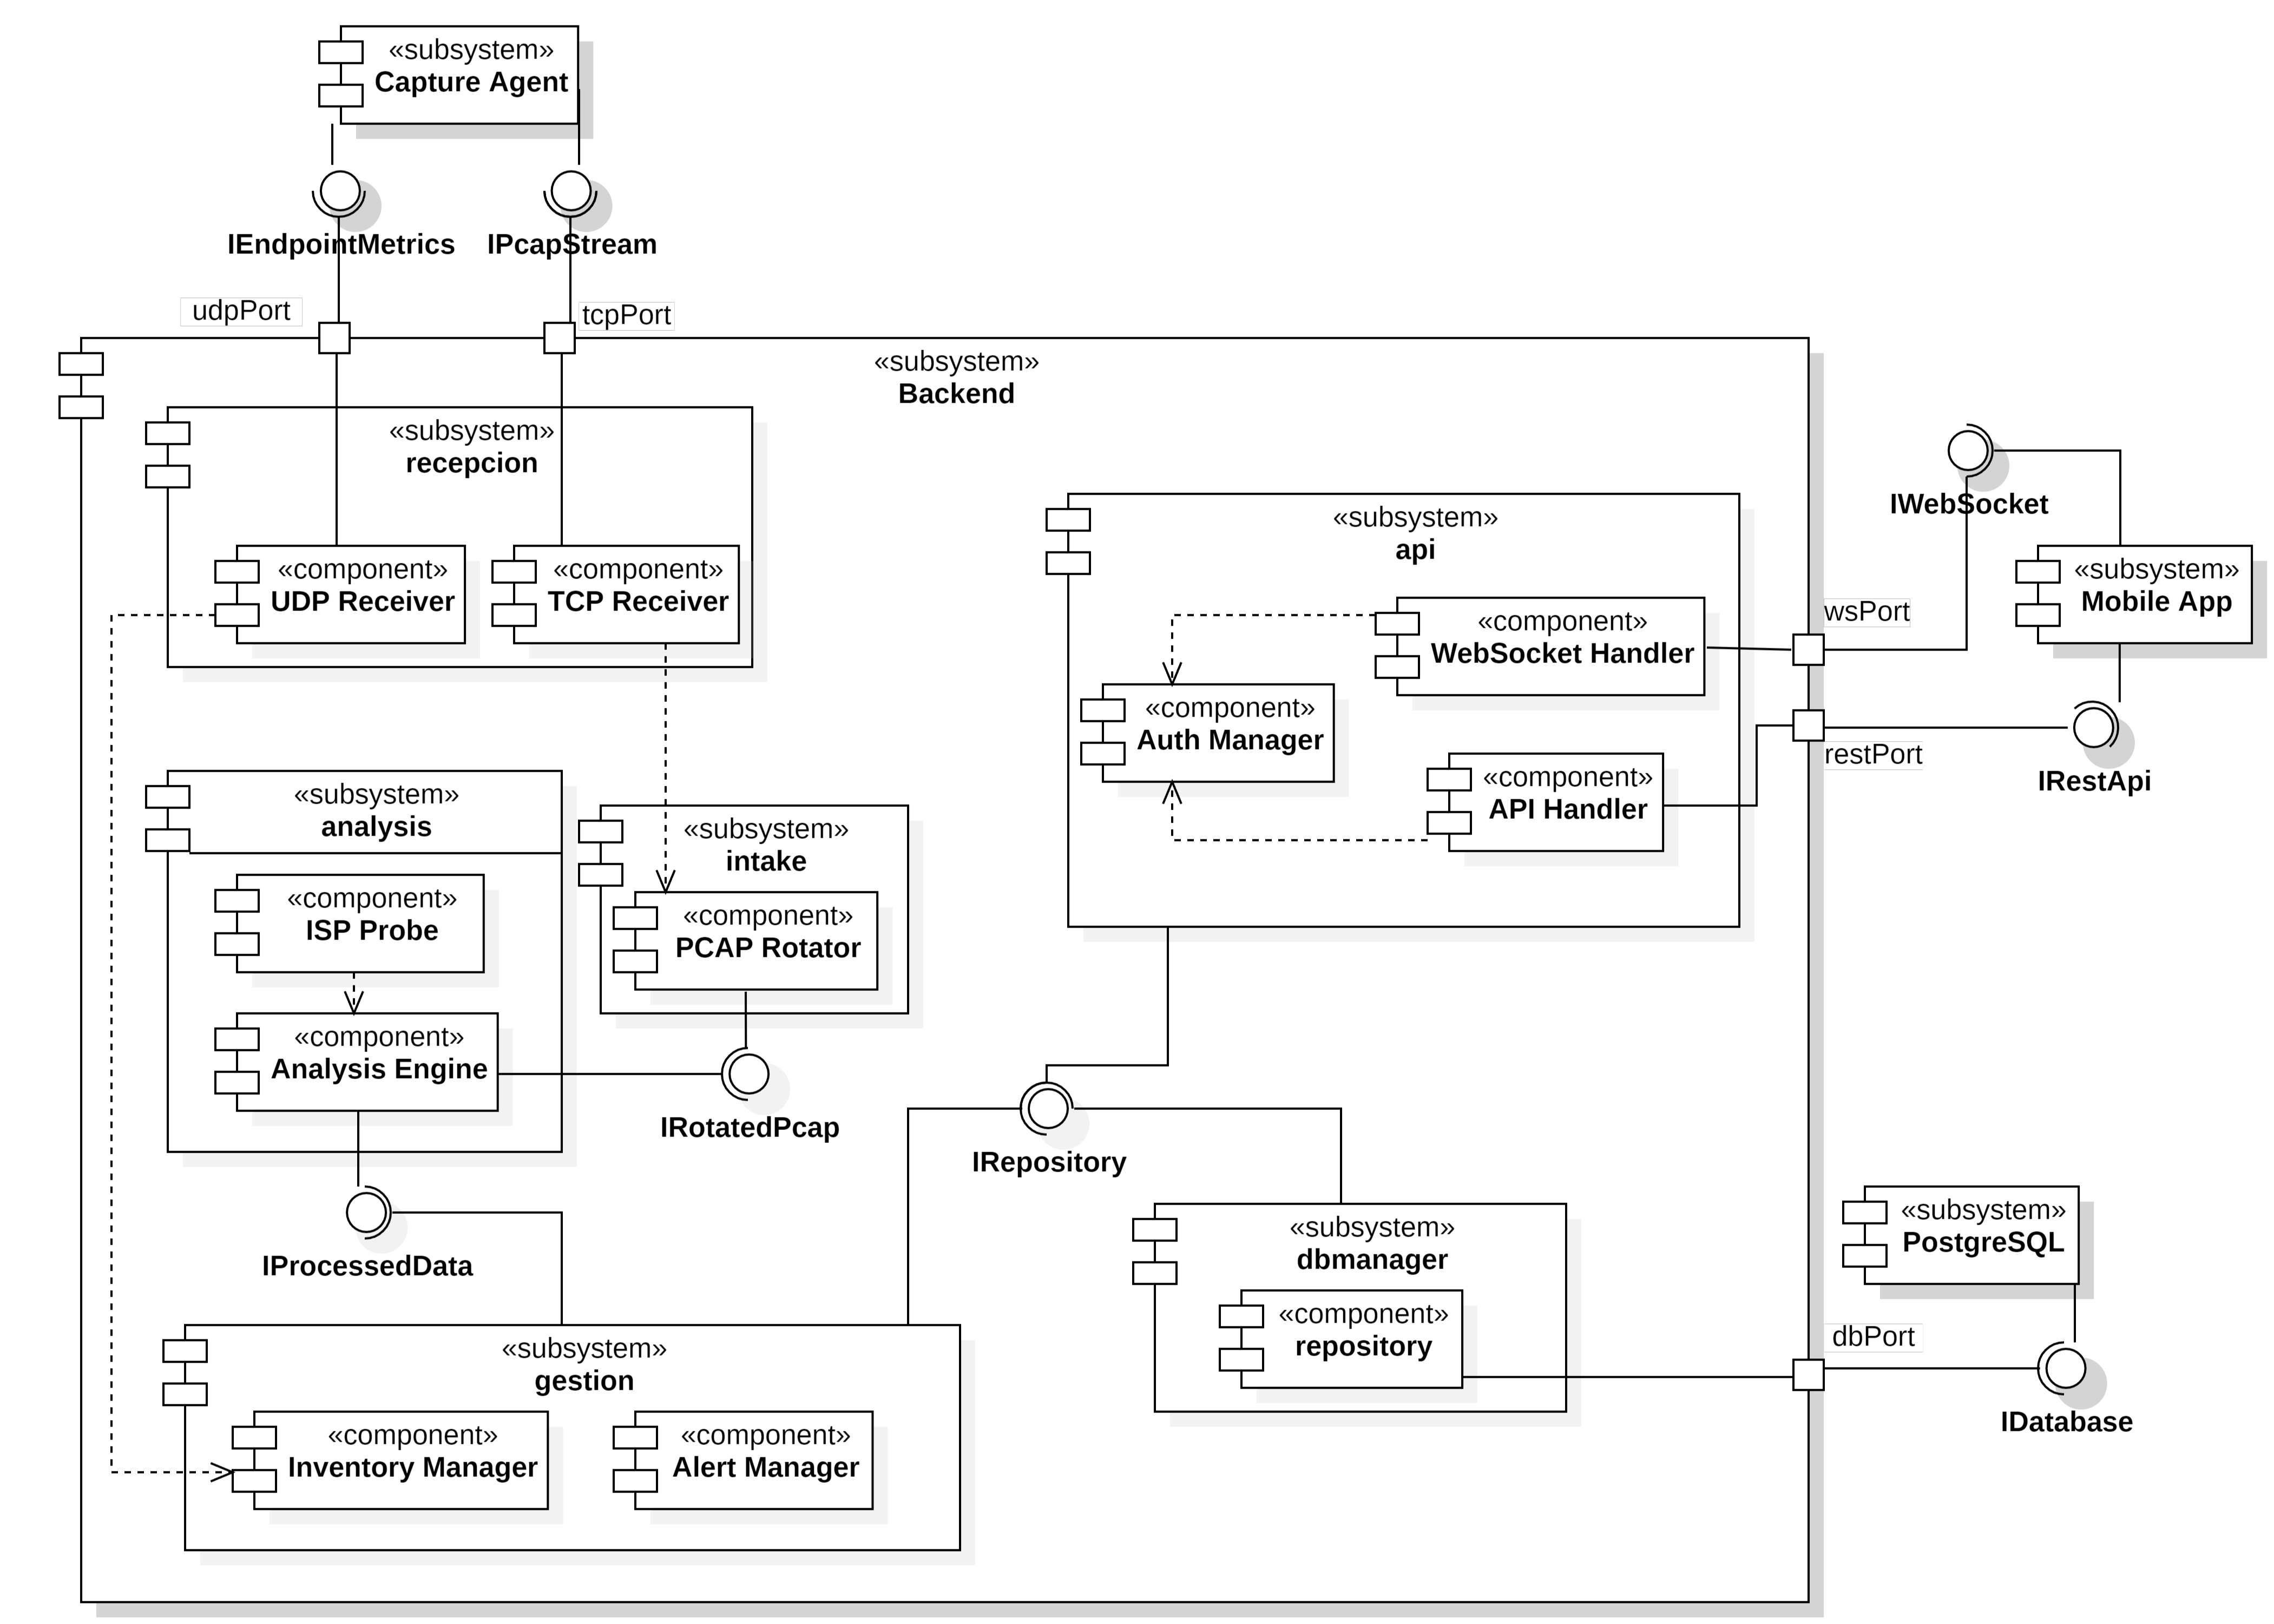
\includegraphics[width=\columnwidth]{diagrama_componentes.png}
\caption{Vista de componentes del sistema (modelo C4 nivel 3). Se muestran los cinco subsistemas internos del backend, las interfaces que exponen y las dependencias entre ellos.}
~\label{fig:componentes}
\end{figure}

La Fig.~\ref{fig:componentes} ilustra la estructura interna del 
backend. El subsistema de recepción (\texttt{UDP Receiver} y 
\texttt{TCP Receiver}) recibe los flujos provenientes de los 
sensores y los entrega a los subsistemas de análisis y almacenamiento 
intermedio. El subsistema de \textit{intake} rota los archivos PCAP 
en ventanas temporales manejables y los pone a disposición del motor 
de análisis mediante la interfaz \texttt{IRotatedPcap}. El subsistema 
de análisis combina la sonda ISP y el motor de análisis principal, 
que procesa los PCAP, genera las métricas contextualizadas y las 
entrega al subsistema de gestión a través de la interfaz 
\texttt{IProcessedData}. El subsistema de gestión consolida el 
inventario de activos y la generación de alertas. Finalmente, el 
subsistema de API, que agrupa el \texttt{Auth Manager}, el 
\texttt{API Handler} y el \texttt{WebSocket Handler}, expone los 
datos persistidos hacia la aplicación móvil. Todos los subsistemas 
acceden a la base de datos PostgreSQL mediante la interfaz 
\texttt{IRepository} expuesta por el subsistema \texttt{dbmanager}.

Esta descomposición responde a dos decisiones arquitectónicas clave. 
La primera es la separación del pipeline de procesamiento y la capa 
de exposición como procesos independientes del sistema operativo, 
comunicados exclusivamente a través de la base de datos compartida 
~\cite{hohpe2003eip}. Esto permite que un fallo en el pipeline no 
afecte la disponibilidad de la API para consultas móviles, y que 
ambos procesos escalen sus recursos de forma independiente según su 
perfil de carga~\cite{silberschatz2018os}. La segunda es el uso de 
interfaces nombradas en el diagrama de componentes, que formalizan 
los contratos entre subsistemas y permiten sustituir implementaciones 
sin afectar al resto del sistema.

\subsubsection{Vista de despliegue}

\begin{figure*}[!t]
\centering
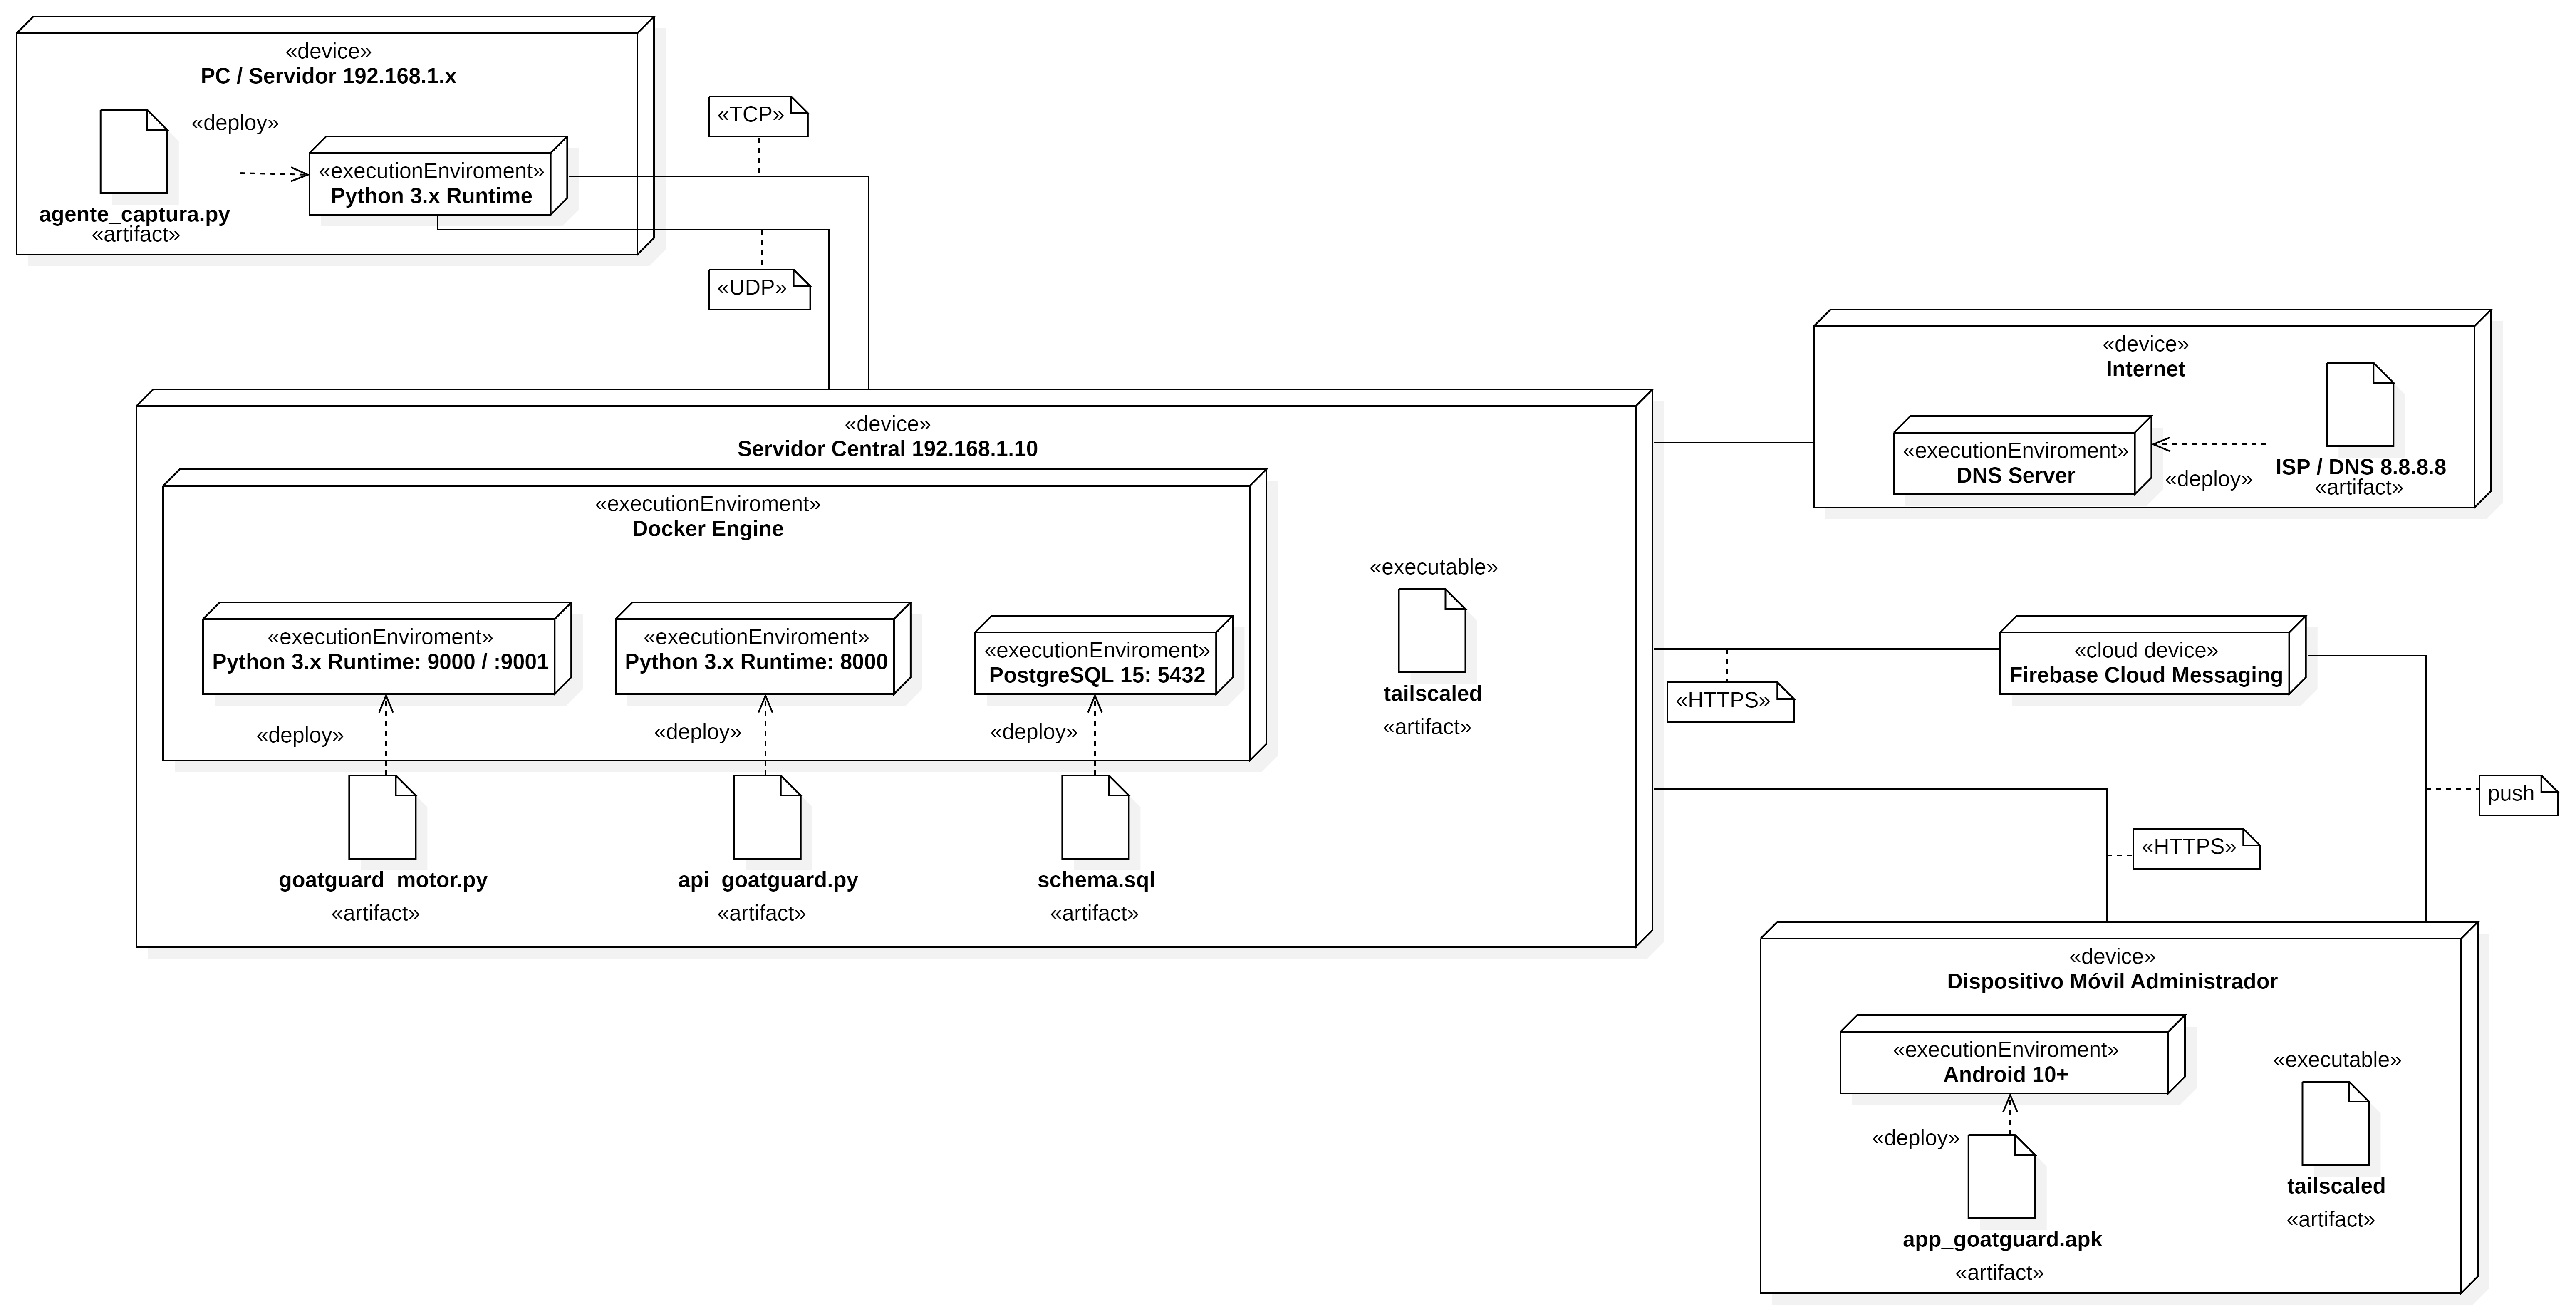
\includegraphics[width=0.95\textwidth]{diagrama_despliegue.png}
\caption{Vista de despliegue del sistema. Los sensores transmiten a un servidor central contenedorizado que expone servicios al dispositivo móvil mediante una red privada Tailscale y al servicio de notificaciones push Firebase Cloud Messaging.}
~\label{fig:diagrama_despliegue}
\end{figure*}

La Fig.~\ref{fig:diagrama_despliegue} presenta la disposición física del 
sistema en su entorno de operación. Los sensores de captura se 
ejecutan como artefactos \texttt{agente\_captura.py} sobre un runtime 
Python 3.x en cada uno de los endpoints de la red local. El servidor 
central, ubicado en la dirección estática 192.168.1.10, aloja tres 
contenedores Docker que ejecutan de forma independiente: el motor de 
pipeline (\texttt{goatguard\_motor.py}) en los puertos 9000 y 9001, 
la API REST (\texttt{api\_goatguard.py}) en el puerto 8000, y el 
servicio PostgreSQL 15 en el puerto 5432. La aplicación móvil, 
empaquetada como \texttt{app\_goatguard.apk}, se ejecuta sobre 
Android 10 o superior en el dispositivo del administrador.



Dos decisiones de despliegue merecen mención explícita. La primera 
es el uso de Tailscale como red privada virtual para conectar el 
dispositivo móvil con el servidor central, lo cual permite al 
administrador consultar el sistema desde fuera de la red local sin 
exponer el servidor a Internet mediante una IP pública. La segunda 
es la integración con Firebase Cloud Messaging para la entrega de 
notificaciones push al dispositivo móvil cuando el motor de análisis 
genera alertas que superan los umbrales de severidad.

\subsubsection{Modelo de datos}

La persistencia del sistema se organiza en torno a tres tipos 
estructurales de entidades que responden a perfiles de acceso 
distintos. Las entidades \textit{base} describen elementos 
relativamente estáticos del dominio cuya información cambia con poca 
frecuencia: una red, un dispositivo, un sensor registrado, un 
usuario autenticado. Las entidades \textit{acumuladas} conservan el 
histórico completo de las mediciones producidas por el motor de 
análisis a lo largo del tiempo; cada ciclo del motor inserta una 
nueva fila por métrica observada, y estas tablas crecen de forma 
monótona hasta que un proceso de retención las recorta. Las 
entidades \textit{sobreescritas} mantienen únicamente el valor más 
reciente de cada métrica y se actualizan mediante operaciones 
\texttt{UPSERT} que sustituyen la fila anterior por la nueva. La 
Fig.~\ref{fig:er-tipologia} ilustra los tres tipos sobre las tablas 
relacionadas con el monitoreo de una red.

\begin{figure}[H]
\centering
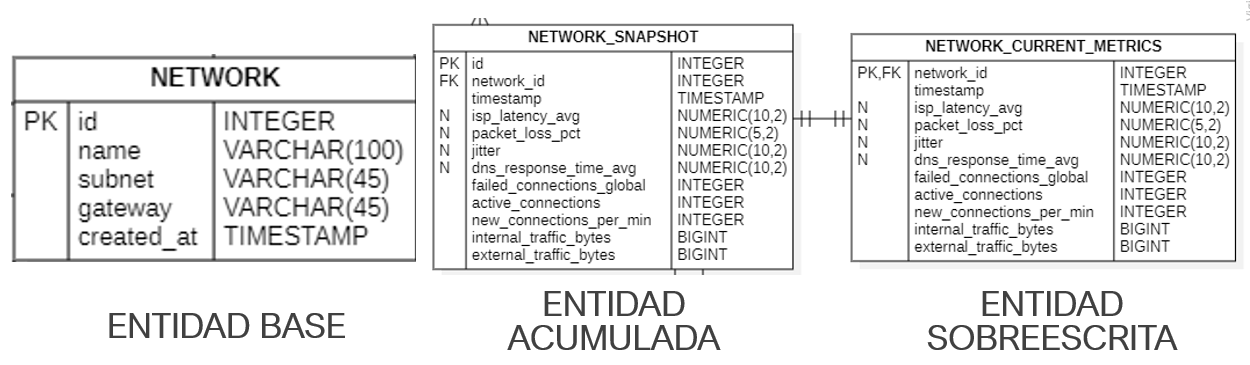
\includegraphics[width=\columnwidth]{er_tipologia.png}
\caption{Tipología de entidades del modelo de datos: \textsc{Network} como entidad base, \textsc{Network\_Snapshot} como entidad acumulada que preserva el histórico, y \textsc{Network\_Current\_Metrics} como entidad sobreescrita que almacena únicamente la última observación.}
~\label{fig:er-tipologia}
\end{figure}

Esta distinción responde a un compromiso entre la necesidad de 
mantener un historial para el análisis retrospectivo y la 
eficiencia de las consultas en tiempo real desde la aplicación 
móvil. Las entidades acumuladas operan como tablas de series 
temporales con inserciones continuas y lecturas analíticas 
ocasionales; su tamaño crece linealmente con el tiempo y requiere 
particionamiento y políticas de retención para mantenerse operativa. 
Las entidades sobreescritas, en contraste, mantienen una sola fila 
por dispositivo y se actualizan en cada ciclo, lo que permite al 
cliente móvil consultar el estado actual de la red en tiempo 
constante sin recorrer el histórico completo. El mismo patrón se 
aplica a los dispositivos (\textsc{Device\_Current\_Metrics} vs 
\textsc{Endpoint\_Snapshot}) y a los top talkers 
(\textsc{Top\_Talker\_Current} vs \textsc{Top\_Talker}).

El conjunto completo de entidades se agrupa en cuatro dominios 
funcionales, como se aprecia en el diagrama completo del modelo 
entidad-relación (Fig.~\ref{fig:er}, ubicada al final del 
documento). El dominio de inventario comprende \textsc{Network}, 
\textsc{Device} y \textsc{Agent}, que describen la estructura 
estática de la red monitoreada. El dominio de mediciones alberga 
las parejas acumulada y sobreescrita de cada tipo de métrica, junto 
con la entidad \textsc{ML\_Prediction} que almacena las 
clasificaciones producidas por el fingerprinting de tráfico. El 
dominio de análisis registra la salida del motor de anomalías: 
\textsc{Alert} para los eventos que superan los umbrales de 
severidad, \textsc{Insight} para las observaciones contextuales 
generadas durante el procesamiento, y \textsc{Top\_Talker} para la 
identificación de los dispositivos de mayor consumo. El dominio de 
autenticación agrupa \textsc{User}, \textsc{Session} y 
\textsc{Push\_Token}, responsables respectivamente de las 
credenciales, los tokens JWT activos y los identificadores para el 
envío de notificaciones push al dispositivo móvil del administrador.

\begin{figure*}[p]
\centering
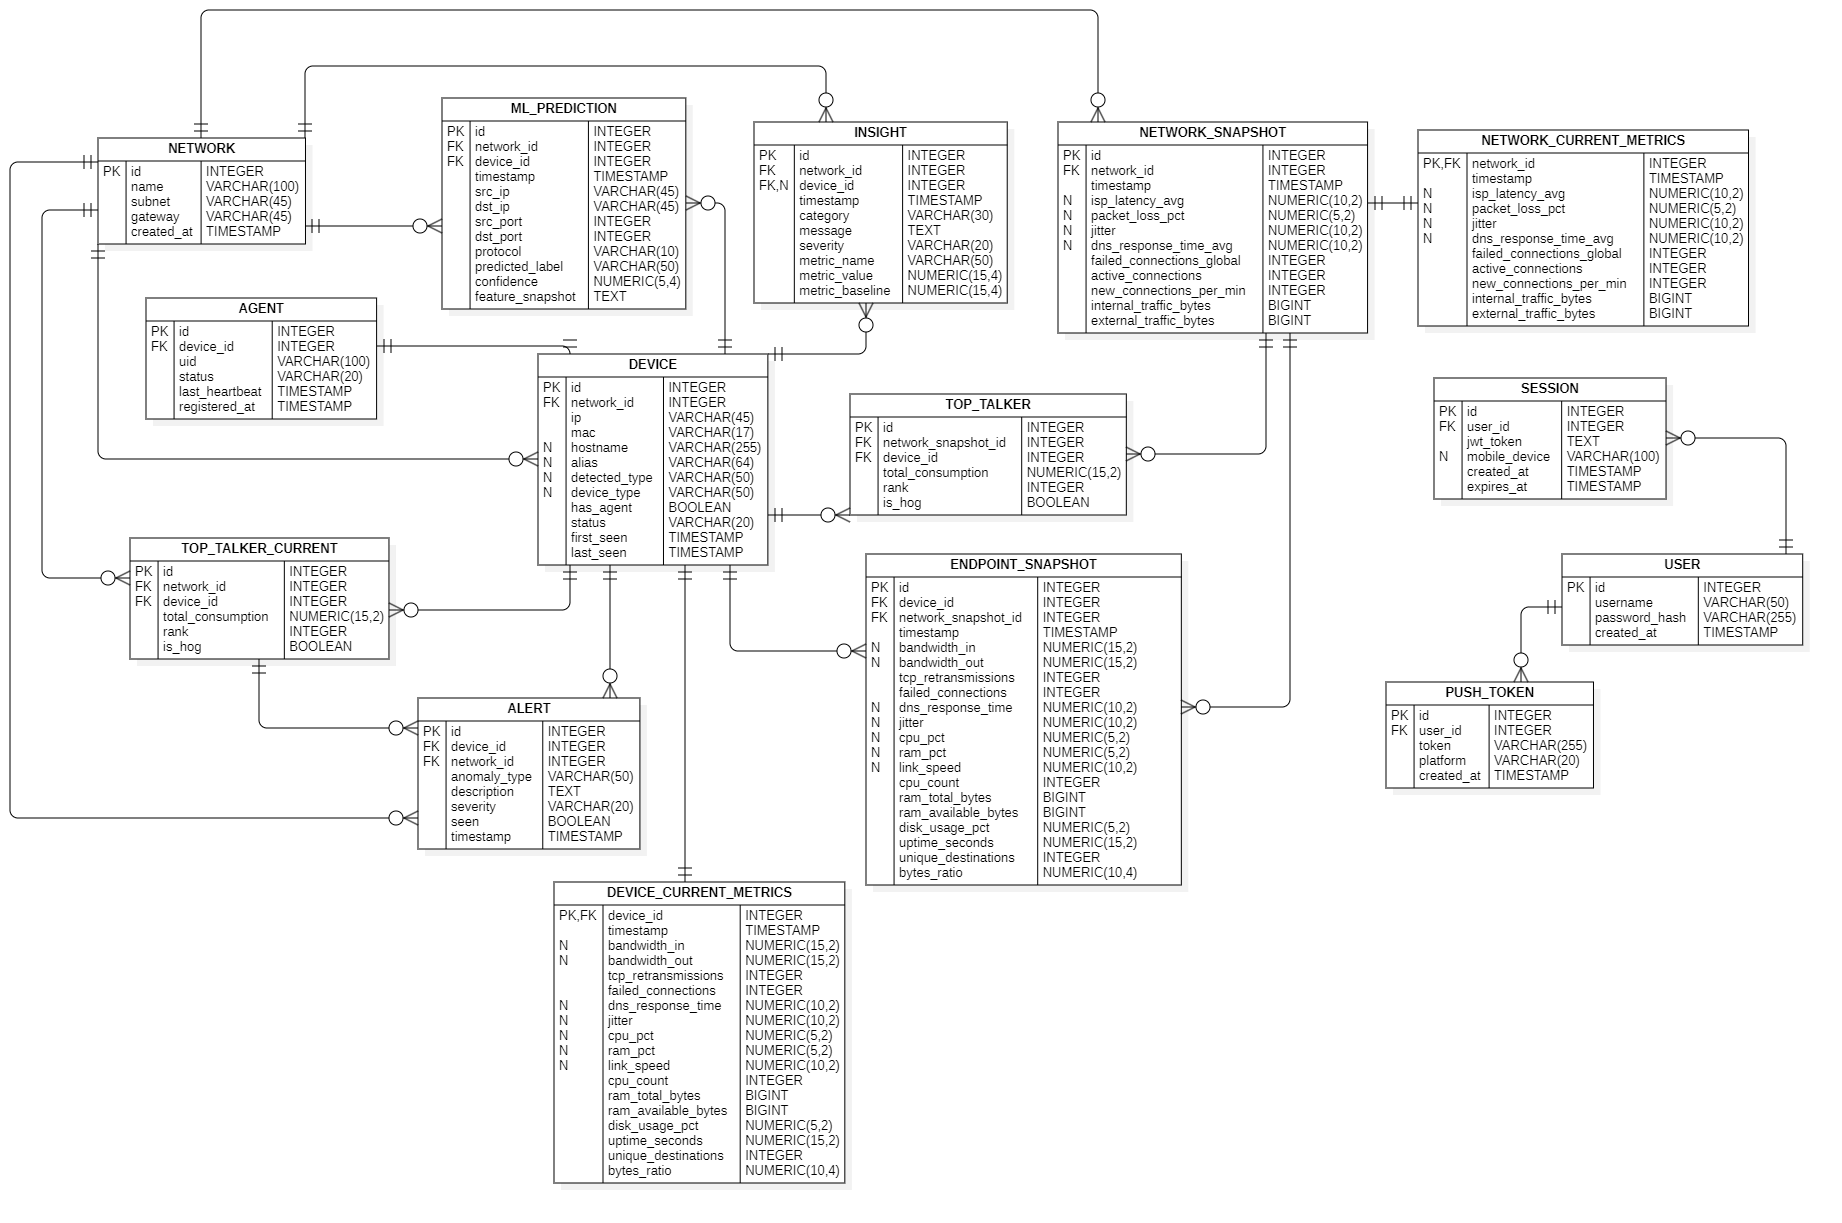
\includegraphics[width=0.95\textwidth]{diagrama_er.png}
\caption{Modelo entidad-relación completo del sistema. Las tablas se agrupan en cuatro dominios funcionales: inventario, mediciones, análisis y autenticación.}
~\label{fig:er}
\end{figure*}

\subsection{Sensor de captura distribuida}
~\label{subsec:sensor}

El sensor de captura es el componente desplegado en cada endpoint 
de la red que observa el tráfico local, recolecta métricas del 
sistema y transmite ambos flujos hacia el backend central. Su 
diseño interno resuelve tres problemas técnicos de forma integrada: 
la captura continua sin bloquear la ejecución de tareas periódicas, 
la sanitización del tráfico antes de su transmisión para preservar 
la confidencialidad de las comunicaciones, y la entrega ordenada de 
paquetes al colector sobre un canal TCP que no preserva fronteras 
entre mensajes.

\subsubsection{Arquitectura interna}

La estructura del sensor (Fig.~\ref{fig:sensor-interno}) se 
organiza en cuatro módulos funcionales: un capturador de paquetes 
que intercepta el tráfico de la interfaz de red seleccionada, un 
sanitizador que aplica el recorte dinámico al payload y preserva la 
longitud original del paquete, un socket TCP que transmite los 
paquetes binarios sanitizados al colector por el puerto 9000, y un 
socket UDP que envía las métricas del endpoint (CPU, memoria RAM, 
disco, velocidad del enlace) serializadas en formato JSON 
~\cite{rfc8259} al puerto 9001.

\begin{figure}[H]
\centering
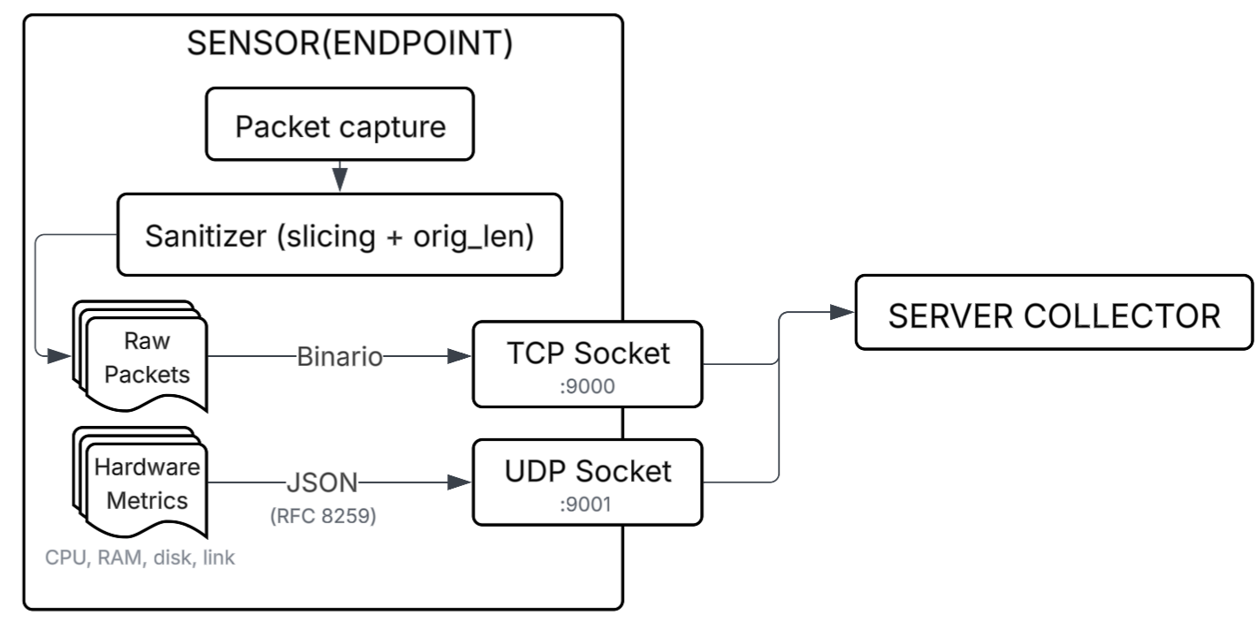
\includegraphics[width=\columnwidth]{sensor_interno.png}
\caption{Arquitectura interna del sensor de captura. El módulo de captura intercepta paquetes, el sanitizador los recorta, y dos sockets independientes transmiten tráfico binario (TCP) y métricas JSON (UDP) al colector.}
~\label{fig:sensor-interno}
\end{figure}

La selección de la interfaz de red principal se realiza de forma 
automática mediante un filtro que descarta las interfaces sin 
conectividad real: las de loopback, las que operan en el rango 
APIPA~\cite{rfc3927} (169.254.0.0/16, indicador de ausencia de 
asignación DHCP), las virtuales de hipervisores y contenedores, y 
los adaptadores Bluetooth. La interfaz seleccionada es aquella que 
posee simultáneamente una dirección IPv4 asignada y una dirección 
MAC asociada, criterio que evidencia conectividad activa a la 
infraestructura de red. El sensor construye su identificador único 
concatenando el hostname del sistema con la dirección MAC de esa 
interfaz, lo que garantiza unicidad a nivel de hardware y legibilidad 
humana en el inventario centralizado.

\subsubsection{Captura concurrente y modelo productor-consumidor}

El sensor ejecuta tareas con perfiles temporales distintos: la 
captura de paquetes es continua y bloqueante, mientras que el 
reporte de métricas y la señal de heartbeat operan en intervalos 
periódicos. La coordinación de estas tareas adopta un modelo de 
concurrencia basado en hilos, siguiendo el patrón productor-consumidor 
descrito por Buschmann et al.~\cite{buschmann1996posa}. Un hilo 
dedicado actúa como productor, invocando la función de captura sobre 
la interfaz seleccionada y depositando cada paquete procesado en un 
buffer intermedio. El hilo principal opera como consumidor, vaciando 
el buffer periódicamente para transmitir los paquetes acumulados al 
colector. La sincronización se implementa mediante exclusión mutua 
sobre el buffer compartido, lo que previene condiciones de carrera 
en el acceso concurrente~\cite{silberschatz2018os}.

El buffer se implementa como una cola acotada con política de 
descarte FIFO.@Cuando la capacidad máxima se alcanza, los paquetes 
más antiguos se descartan para acomodar los nuevos. Esta decisión 
protege la disponibilidad del endpoint frente a escenarios donde el 
consumidor no puede vaciar el buffer a la velocidad necesaria, como 
ocurre ante una pérdida temporal de conectividad con el colector: 
el consumo de memoria del sensor permanece acotado y predecible, en 
cumplimiento del requerimiento no funcional de rendimiento que 
establece un consumo máximo de memoria por sensor.

\subsubsection{Sanitización del tráfico}

El tráfico capturado no se transmite en su forma original al 
colector. Antes de su almacenamiento en el buffer, cada paquete 
atraviesa el sanitizador, que aplica un recorte dinámico al payload 
en función del puerto de destino del flujo. Los encabezados de las 
capas de enlace, red y transporte (aproximadamente 54 bytes, según 
se justificó en la Sección~\ref{sec:marco-teorico}) contienen toda 
la información necesaria para reconstruir flujos y extraer métricas 
de comportamiento, de modo que un recorte a 96 bytes preserva la 
totalidad de las cabeceras con margen para opciones TCP 
~\cite{stevens2004unix}. Para tráfico dirigido a los puertos 
asociados a DNS (53) y HTTPS (443), el recorte se extiende a 300 
bytes; este margen adicional captura el dominio consultado en el 
caso de DNS~\cite{rfc1035} y la indicación de nombre de servidor 
(SNI) del handshake TLS en el caso de HTTPS~\cite{rfc8446}, 
elementos con valor diagnóstico que no comprometen el contenido de 
las comunicaciones.

Cada paquete sanitizado conserva un campo \texttt{orig\_len} con la 
longitud original antes del truncamiento. Este campo es necesario 
para que el motor de análisis calcule métricas volumétricas como 
throughput, bytes por flujo, tamaño promedio de paquete y carga del 
enlace sobre el volumen real de tráfico, no sobre el volumen 
truncado. La sanitización materializa así el principio de 
minimización de datos exigido por el marco legal descrito en la 
Sección~\ref{sec:marco-legal}: se preserva exclusivamente la 
información técnica necesaria para el análisis, eliminando el 
contenido de las comunicaciones que podría constituir interceptación 
indebida.

\subsubsection{Protocolo binario de transporte}

TCP, como protocolo orientado a flujo de bytes, no preserva las 
fronteras entre los mensajes individuales emitidos por el transmisor 
~\cite{rfc793}. Un envío de 116 bytes por parte del sensor puede ser 
recibido por el colector como una lectura de 80 bytes seguida de 
otra de 36, o como una única lectura de 116, dependiendo del estado 
del buffer del kernel y de las condiciones de la red. Esta 
característica, conocida como \textit{message boundary problem} 
~\cite{stevens2004unix}, requiere que el protocolo de aplicación 
implemente su propio mecanismo de delimitación (Fig. 
~\ref{fig:message-boundary}).

\begin{figure}[H]
\centering
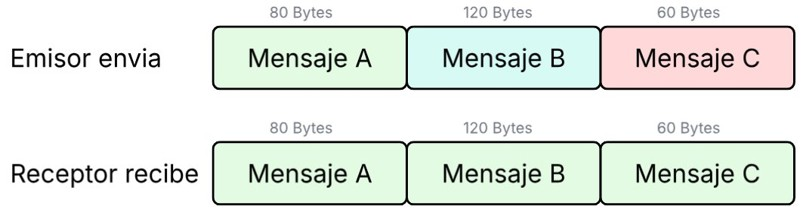
\includegraphics[width=\columnwidth]{tcp_framing.jpg}
\caption{Problema de fronteras en TCP y solución mediante \textit{length-prefix framing}. El receptor no puede inferir los límites de los mensajes originales sin un esquema explícito de delimitación. El prefijo de longitud antepuesto a cada payload resuelve la ambigüedad.}
~\label{fig:message-boundary}
\end{figure}

El sensor resuelve este problema mediante un esquema de 
\textit{length-prefix framing}: antepone a cada paquete capturado un 
encabezado fijo de 20 bytes que permite al receptor delimitar los 
mensajes dentro del flujo continuo de TCP.@El encabezado se 
estructura en \textit{network byte order} (big endian, conforme a 
RFC 793) y contiene cuatro campos (Fig.~\ref{fig:tcp-header}): la 
longitud original del paquete antes de la sanitización 
(\texttt{orig\_len}, 4 bytes), el puerto destino extraído de la 
cabecera de transporte del paquete capturado (\texttt{dst\_port}, 4 
bytes), la marca temporal de captura en formato IEEE 754 de doble 
precisión (\texttt{timestamp}, 8 bytes), y la longitud de los datos 
truncados que siguen al encabezado (\texttt{data\_len}, 4 bytes).

\begin{figure}[H]
\centering
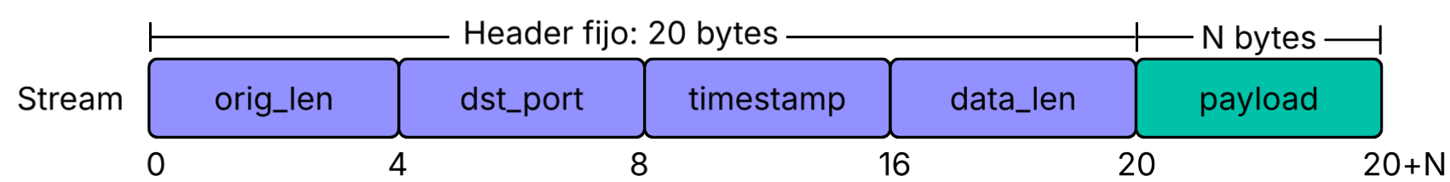
\includegraphics[width=\columnwidth]{tcp_header.png}
\caption{Estructura del encabezado binario de transporte sensor-colector. Los 20 bytes de cabecera preceden a un payload de tamaño variable indicado por \texttt{data\_len}.}
~\label{fig:tcp-header}
\end{figure}

\subsubsection{Transporte dual y fundamentación de protocolos}

La separación del tráfico capturado (TCP) y las métricas del sistema 
(UDP) en dos canales paralelos responde a la diferencia en los 
requisitos de confiabilidad de cada tipo de dato. Los paquetes de red 
capturados son irrecuperables: cada paquete representa un evento 
único en la red, y si se pierde en tránsito no existe otra copia ni 
se regenera en el siguiente ciclo. La garantía de entrega ordenada y 
confiable que TCP proporciona mediante sus mecanismos de 
acknowledgement, retransmisión y control de flujo~\cite{rfc793} es 
por tanto apropiada para este canal. Las métricas del endpoint, en 
contraste, son tolerantes a pérdida: se generan periódicamente cada 
cinco segundos, cada paquete contiene una muestra completa del 
estado actual del sistema, y si un paquete UDP~\cite{rfc768} se 
pierde, el siguiente lo reemplaza con datos más recientes. La 
retransmisión de una métrica obsoleta consumiría ancho de banda sin 
aportar valor. El sobrecosto de ocho bytes de encabezado UDP frente 
a los veinte mínimos de TCP~\cite{stevens2004unix}, sumado a la 
ausencia de establecimiento de sesión, hace de UDP la elección 
natural para este perfil de transmisión.

\subsection{Backend centralizado y pipeline de análisis}
~\label{subsec:backend}

El backend recibe los flujos provenientes de los sensores y los 
transforma en métricas contextualizadas que alimentan el inventario 
dinámico, el motor de anomalías y la capa de exposición. Su diseño 
interno obedece al patrón arquitectónico de \textit{Pipes and 
Filters}~\cite{buschmann1996posa}: los datos atraviesan una 
secuencia de etapas especializadas conectadas por interfaces 
tipadas, y cada etapa opera sobre la salida estructurada de la 
anterior sin conocer su implementación. La Fig.~\ref{fig:servidor-central} 
ilustra esta cadena completa, desde los 
receptores TCP\@ que aceptan los flujos de los sensores hasta el 
repositorio que persiste las métricas resultantes en PostgreSQL\@.

\begin{figure}[H]
\centering
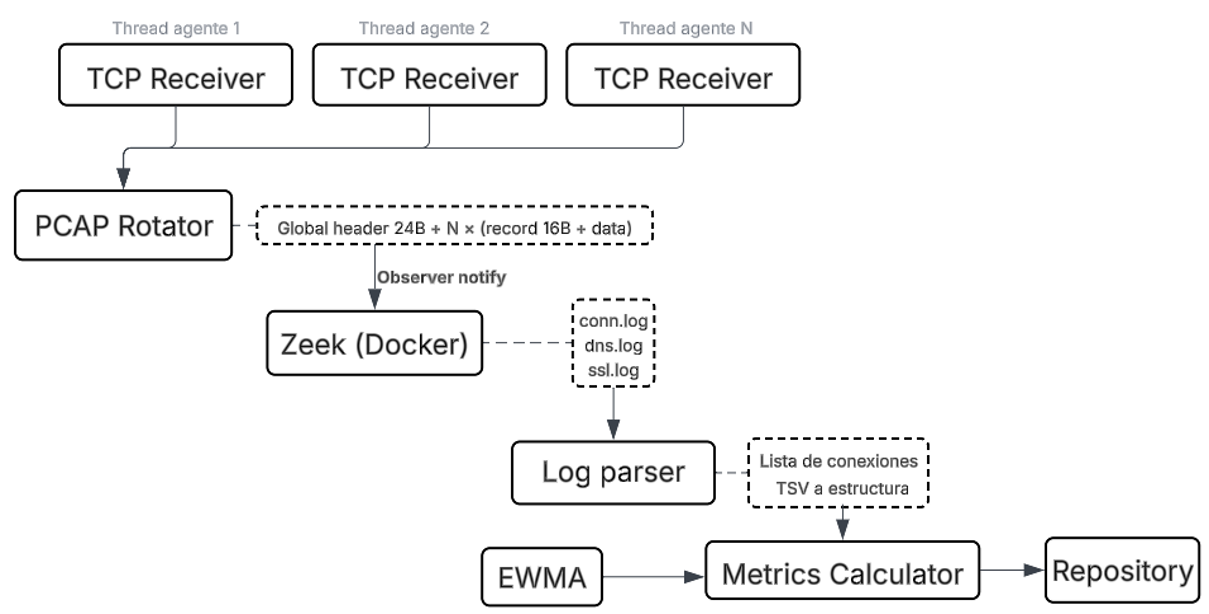
\includegraphics[width=\columnwidth]{servidor_central.png}
\caption{Pipeline interno del servidor central. Los receptores TCP aceptan los flujos de los sensores en hilos independientes; el rotador fragmenta el tráfico en archivos PCAP de ventana temporal fija; Zeek los procesa y genera logs; el parser los convierte en estructuras de conexión; el calculador aplica EWMA para derivar métricas contextualizadas, y el repositorio las persiste.}
\label{fig:servidor-central}
\end{figure}

\subsubsection{Recepción concurrente de flujos}

El servidor colector opera como punto de convergencia de datos en 
una arquitectura distribuida en la que múltiples sensores 
transmiten simultáneamente hacia el mismo destino. La concurrencia 
en el receptor es un requisito funcional: el servidor debe atender 
múltiples flujos de ingreso sin que el procesamiento de un sensor 
bloquee la recepción de datos provenientes de otros.

El modelo de concurrencia adoptado se basa en el patrón 
\textit{Thread-per-Client}~\cite{schmidt2000posa2}. Un hilo 
principal ejecuta un ciclo de aceptación de conexiones mediante la 
primitiva \texttt{accept()} del API\@ de sockets Berkeley~\cite{stevens2004unix}. 
Esta primitiva opera de forma bloqueante: 
suspende la ejecución del hilo hasta que un sensor inicia una 
conexión mediante el \textit{three-way handshake} de TCP~\cite{rfc793}. 
Al completarse el handshake, \texttt{accept()} 
retorna un descriptor de socket exclusivo para esa conexión, 
mientras el socket original permanece en estado de escucha para 
conexiones subsiguientes. Por cada conexión aceptada se instancia 
un hilo dedicado que ejecuta la lógica de lectura del protocolo 
binario descrito en la Sección~\ref{subsec:sensor}. El aislamiento 
entre hilos garantiza que la latencia o desconexión de un sensor no 
afecte la recepción de datos provenientes de los demás.

La elección de Thread-per-Client sobre alternativas como la 
multiplexación de E/S mediante \texttt{select()} o \texttt{epoll()}~\cite{stevens2004unix} 
se fundamenta en el número acotado de 
sensores previstos por los requerimientos no funcionales de 
rendimiento del sistema. Para esta escala, la simplicidad del 
modelo de hilos supera las ganancias de rendimiento que los 
mecanismos de E/S asíncronos ofrecen en escenarios de alta 
concurrencia con miles de conexiones simultáneas.

Los hilos se configuran como \textit{daemon threads}, lo que 
asegura su terminación automática cuando el proceso principal del 
servidor finaliza. Esta configuración previene la persistencia de 
hilos huérfanos que consumirían recursos del sistema operativo sin 
propósito tras un apagado controlado~\cite{silberschatz2018os}.

\subsubsection{Segmentación del tráfico en archivos PCAP}

El receptor TCP reconstruye los paquetes sanitizados emitidos por 
cada sensor y los entrega al \textit{PCAP Rotator}, el primer 
filtro del pipeline. Este componente acumula los paquetes recibidos 
en archivos con formato PCAP estándar~\cite{harris2020libpcap}, 
compuestos por un encabezado global de 24 bytes seguido de una 
secuencia de registros donde cada uno consta de un encabezado de 16 
bytes y el contenido del paquete. Este formato es el esperado por 
las herramientas convencionales de análisis de tráfico, lo que 
permite que componentes externos especializados procesen la salida 
sin necesidad de transformaciones intermedias.

La rotación obedece a una ventana temporal fija: cada archivo PCAP 
acumula el tráfico de un intervalo acotado, tras el cual se cierra 
y se emite una notificación al motor de análisis. Esta 
notificación se implementa siguiendo el patrón \textit{Observer}~\cite{gof1994}, 
que desacopla al productor del consumidor de 
eventos: el rotador publica la finalización de cada ventana sin 
necesidad de conocer qué componentes la procesarán, y el motor de 
análisis se suscribe a estas notificaciones para incorporar el 
archivo recién cerrado a su cola de trabajo. El resultado es una 
cadena donde la cadencia de análisis queda determinada por la 
ventana de rotación, no por el ritmo de llegada de los paquetes.

\subsubsection{Análisis de protocolos con Zeek}

El motor de análisis delega el procesamiento semántico del tráfico 
a Zeek, un framework de análisis de tráfico de red ampliamente 
utilizado en el ámbito de la seguridad informática~\cite{paxson1999zeek}. 
A diferencia de los analizadores orientados 
a firmas, Zeek opera sobre el comportamiento de los protocolos: 
reconstruye sesiones TCP, identifica los protocolos de aplicación 
mediante inspección de contenido, y produce registros estructurados 
que describen cada conexión en términos de sus partes, su duración, 
los bytes intercambiados en cada dirección y los metadatos 
específicos del protocolo detectado.

Cada archivo PCAP emitido por el rotador se entrega a una instancia 
de Zeek ejecutada en un contenedor Docker aislado del resto del 
sistema. Esta aislación cumple dos propósitos. El primero es de 
seguridad: el procesamiento de paquetes arbitrarios provenientes 
de una red real plantea riesgos de explotación de vulnerabilidades 
en el propio analizador, y la ejecución en contenedor acota el 
dominio de compromiso en caso de fallo. El segundo es operativo: 
Zeek y sus dependencias se mantienen versionadas de forma 
independiente del resto del backend, lo que simplifica las 
actualizaciones y garantiza la reproducibilidad del entorno de 
análisis.

Zeek produce múltiples archivos de registro por cada archivo PCAP 
procesado. Los relevantes para el pipeline son \texttt{conn.log}, 
que describe cada conexión observada con su 
tupla de direcciones y puertos, marcas temporales, duración y 
conteos de bytes y paquetes en cada sentido; \texttt{dns.log}, que 
registra las consultas y respuestas DNS junto con los tiempos de 
respuesta; y \texttt{ssl.log}, que describe los handshakes TLS 
incluyendo el nombre de servidor indicado (SNI) cuando está 
presente.

\subsubsection{Transformación de logs y cálculo de métricas}

Los archivos de registro producidos por Zeek son ficheros de texto 
tabular (TSV) que no son aptos para el análisis en memoria de 
aplicaciones posteriores. El \textit{Log Parser} actúa como 
segundo filtro del pipeline: recorre los logs, filtra las columnas 
relevantes y convierte cada línea en una estructura de datos 
tipada que representa una conexión individual. Esta estructura 
homogénea permite que el componente siguiente opere sin necesidad 
de manipular texto crudo.

El \textit{Metrics Calculator} consume las estructuras de conexión 
y deriva las métricas contextualizadas que constituyen el producto 
del pipeline. Entre ellas, el ancho de banda entrante y saliente 
por dispositivo, la tasa de retransmisiones TCP, el tiempo de 
respuesta DNS, el número de conexiones activas y fallidas, y la 
clasificación de \textit{top talkers} dentro de la ventana 
analizada. Las métricas que requieren suavizado temporal se 
computan mediante el método EWMA~\cite{lucas1990ewma,roberts1959ewma}, 
cuyo detalle formal se desarrolla en la Sección~\ref{subsec:motor} 
junto con la descripción del motor de detección de anomalías.

\subsubsection{Persistencia y separación de procesos}

Las métricas resultantes se entregan al \textit{Repository}, un 
componente que encapsula el acceso a PostgreSQL y expone una 
interfaz uniforme hacia el resto del backend. La escritura 
distingue entre entidades acumuladas y sobreescritas, según la 
tipología del modelo de datos descrita en la Sección~\ref{subsec:arquitectura}: 
cada ciclo inserta una nueva fila en 
las tablas \textsc{\_Snapshot} y actualiza mediante \texttt{UPSERT} 
las tablas \textsc{\_Current\_Metrics}.

La comunicación entre el pipeline de procesamiento y la capa de 
exposición (API REST y WebSocket, Sección~\ref{subsec:api}) se 
realiza exclusivamente a través de la base de datos, sin 
comunicación directa entre los dos procesos. Este patrón, 
conocido como \textit{Shared Database} en la literatura de 
integración empresarial~\cite{hohpe2003eip}, es apropiado cuando 
ambos extremos pertenecen a la misma organización y comparten el 
modelo de datos, y aporta dos ventajas. La primera es de 
aislamiento de fallos: un bloqueo o reinicio del pipeline no 
afecta la disponibilidad de la API para consultas móviles, y 
viceversa. La segunda es de escalabilidad independiente: ambos 
procesos pueden ajustar sus recursos asignados según su perfil de 
carga específico, que es distinto en cada caso. El pipeline opera 
en ráfagas periódicas con alto consumo de CPU, mientras que la 
API presenta un perfil de carga irregular dominado por la 
frecuencia de consulta desde el cliente móvil.

\subsection{Motor de detección de anomalías}
~\label{subsec:motor}

El motor de detección opera como consumidor de las métricas 
contextualizadas producidas por el pipeline descrito en la Sección~\ref{subsec:backend} 
y convierte cada observación en una 
evaluación cualitativa sobre su desviación respecto al comportamiento 
habitual del dispositivo. El diseño del motor se fundamenta en tres 
decisiones articuladas: un baseline adaptativo por dispositivo y por 
métrica mediante EWMA, una cuantificación de desviaciones mediante 
Z-Score adaptativo sobre varianza móvil, y un filtro de persistencia 
que exige confirmación temporal antes de generar una alerta. La 
justificación teórica de esta combinación y las limitaciones de las 
alternativas consideradas se desarrollaron en la Sección~\ref{sec:marco-teorico}; 
la presente subsección describe las 
decisiones concretas de parametrización y los detalles algorítmicos 
adoptados en la implementación.

\subsubsection{Baseline adaptativo por dispositivo}

Cada par dispositivo-métrica mantiene dos variables de estado: la 
media exponencial~\(\mu_t\) y la varianza exponencial~\(\sigma^2_t\). 
En cada ciclo de análisis (30~segundos), el motor recibe el vector 
de métricas actuales y actualiza estas dos variables mediante las 
recurrencias
\begin{equation}
\mu_t = \alpha\, x_t + (1-\alpha)\, \mu_{t-1}
\label{eq:ewma-impl}
\end{equation}
\begin{equation}
\sigma^2_t = (1-\alpha)\bigl[\sigma^2_{t-1} + \alpha(x_t - \mu_{t-1})^2\bigr]
\label{eq:ewmv-impl}
\end{equation}
con factor de suavizado~\(\alpha = 0{,}10\)~\cite{lucas1990ewma,roberts1959ewma}. 
Esta elección equilibra estabilidad y reactividad: el peso que una 
observación de hace~\(k\) ciclos retiene en el baseline decae como~\(\alpha(1-\alpha)^k\), 
de modo que una observación emitida hace 
siete ciclos (aproximadamente tres minutos y medio) conserva la mitad 
de su peso original, y una observación de hace 44 ciclos (22 minutos) 
retiene menos del uno por ciento. Más allá de esa ventana el histórico 
está efectivamente olvidado, lo que permite al motor adaptarse a 
cambios legítimos de régimen en cuestión de minutos, a diferencia del 
Z-Score con media acumulada, que requeriría horas para converger al 
nuevo nivel.

Un factor de suavizado menor (por ejemplo~\(\alpha = 0{,}01\)) 
produciría un baseline con memoria superior a cuatro horas, 
demasiado lento para adaptarse a cambios operativos legítimos de los 
dispositivos monitoreados. Un factor mayor (por ejemplo~\(\alpha = 0{,}50\)) 
produciría un baseline con memoria de tres minutos, tan 
reactivo que una anomalía sostenida se absorbería en el propio 
baseline antes de que el sistema alcanzara a reportarla con su 
magnitud completa. El valor~\(\alpha = 0{,}10\) sitúa el motor en 
un punto intermedio validado empíricamente sobre las 12~métricas 
monitoreadas por dispositivo.

\subsubsection{Varianza mínima y evaluación antes de actualización}

Dos detalles de implementación tienen consecuencias sobre el 
comportamiento del detector y merecen explicitación. El primero es 
la existencia de un piso mínimo de varianza configurado según la 
escala de cada métrica: 1{,}0 para las expresadas en porcentaje, 
100{,}0 para las expresadas en bytes por segundo, 0{,}5 para los 
conteos, 0{,}01 para los ratios y 0{,}1 para las métricas de 
latencia. Este piso se emplea en el denominador del Z-Score cuando 
la varianza acumulada cae por debajo, lo que ocurre con métricas que 
permanecen constantes durante períodos largos (por ejemplo, una tasa 
de pérdida de paquetes que se mantiene en cero durante horas) y que, 
sin ese piso, producirían Z-Scores artificialmente grandes ante 
cualquier fluctuación legítima posterior.

El segundo detalle concierne al orden de evaluación y actualización 
dentro de cada ciclo. El Z-Score se calcula contra el baseline y la 
varianza del ciclo anterior, 
\begin{equation}
Z_t = \frac{x_t - \mu_{t-1}}{\sqrt{\sigma^2_{t-1} + \varepsilon}}
\label{eq:zscore-impl}
\end{equation}
antes de actualizar esas variables con el valor observado. El 
invertir el orden haría que la anomalía se absorbiera parcialmente 
en el baseline antes de ser evaluada, reduciendo artificialmente su 
Z-Score y comprometiendo la detección. En las pruebas del sistema, 
un valor de~\(\mathtt{cpu\_pct} = 45\%\) contra un baseline de~\(15\%\) 
produce~\(Z \approx 30{,}4\) cuando se evalúa antes de 
actualizar; si se actualizaran primero el baseline y la varianza, el 
mismo valor produciría~\(Z < 3\). La evaluación anticipada preserva 
la sensibilidad completa del detector.

\subsubsection{Fase de calentamiento}

Durante los primeros 30~ciclos de observación (15~minutos) sobre un 
dispositivo nuevo, el motor acumula muestras y actualiza el baseline 
y la varianza, pero no genera alertas. La razón es cuantitativa: con 
pocas observaciones, la varianza es cercana a cero porque aún no se 
ha observado suficiente variabilidad natural. Un dispositivo cuya 
\(\mathtt{cpu\_pct}\) oscila legítimamente entre el 10~\% y el 
20~\% tendría, tras cinco ciclos, una varianza mínima; si el sexto 
valor es~22~\% (dentro del rango normal), el Z-Score explotaría a 
valores artificialmente altos porque la desviación estándar en el 
denominador sería casi nula. La ventana de 30~ciclos garantiza que 
la varianza refleje la variabilidad real del dispositivo antes de 
habilitar las alertas. Si un dispositivo se desconecta 
temporalmente y reconecta, su baseline se conserva en memoria y no 
reinicia la fase de calentamiento, dado que la desconexión no 
invalida el perfil de comportamiento previamente establecido.

\subsubsection{Clasificación de severidad}

Una vez superada la fase de calentamiento, cada ciclo produce para 
cada métrica un valor de~\(|Z_t|\) que el motor clasifica según tres 
umbrales de severidad. Las observaciones con~\(|Z_t| < 1{,}5\) se 
consideran dentro del rango normal. Aquellas con~\(1{,}5 \leq |Z_t| < 2{,}0\) 
se clasifican como informativas: se registran en la tabla 
\textsc{Insight} para análisis retrospectivo pero no generan 
notificación. Las que cumplen~\(2{,}0 \leq |Z_t| < 3{,}0\) se 
clasifican como \textit{warning}: representan desviaciones con 
probabilidad de ocurrencia de aproximadamente 4{,}56~\% bajo una 
distribución normal, una de cada 22~observaciones esperadas. Las 
que superan~\(|Z_t| \geq 3{,}0\) se clasifican como \textit{critical}: 
probabilidad de aproximadamente 0{,}27~\%, una de 
cada 370~observaciones~\cite{montgomery2013spc}. Esta gradación 
permite que cada alerta incluya una cuantificación estadística de su 
rareza, no únicamente una clasificación binaria.

\subsubsection{Filtro de persistencia}

Si cada observación con~\(|Z_t| \geq 2{,}0\) generara una alerta 
inmediata, el sistema producirían un volumen elevado de falsas 
alarmas ante fluctuaciones transitorias que son parte del 
comportamiento normal de una red LAN:@ráfagas momentáneas de 
tráfico, picos puntuales de respuesta DNS, o variaciones breves de 
latencia. Estas oscilaciones no son anomalías en el sentido 
operativo: no requieren intervención porque se resuelven por sí 
solas en el siguiente ciclo. Las anomalías reales, en contraste, se 
caracterizan por persistir durante varios ciclos consecutivos.

Para discriminar entre fluctuaciones transitorias y anomalías 
sostenidas, el motor incorpora un filtro de persistencia de 
parámetros~\(N\)~y~\(M\) en el espíritu de las reglas de Western 
Electric para cartas de control~\cite{montgomery2013spc}. El filtro 
exige que~\(|Z_t| \geq 2{,}0\) se cumpla en al menos~\(N\) de los 
últimos~\(M\) ciclos para emitir una alerta. Valores ensayados sobre 
datos sintéticos con anomalías conocidas muestran que configuraciones 
demasiado permisivas (sin filtro, o~\(N/M = 2/4\)) generan cientos 
de falsas alarmas frente a decenas de anomalías reales, mientras que 
configuraciones demasiado estrictas (\(N/M = 3/3\) o~\(3/5\)) pierden 
entre 40~\% y 45~\% de las anomalías reales.

La configuración~\(N/M = 2/2\) adoptada en el sistema exige que la 
desviación se mantenga en dos ciclos consecutivos (un minuto) antes 
de emitir la alerta. Sobre las pruebas sintéticas, esta 
configuración reduce las falsas alarmas de 383 (sin filtro) a 16, 
una disminución del 96~\%, mientras preserva 45 de las 48 anomalías 
reales inyectadas, es decir, una tasa de detección del 93{,}8~\%. 
Esta relación entre tasa de detección y tasa de falsas alarmas es la 
que justifica la elección operativa del filtro.

\subsubsection{Ciclo completo y persistencia de alertas}

El ciclo del motor se ejecuta cada 30~segundos. En cada iteración, 
para cada par dispositivo-métrica activo, el motor recupera el 
estado previo de~\(\mu_{t-1}\) y~\(\sigma^2_{t-1}\) desde memoria, 
evalúa el Z-Score contra el valor observado, actualiza el baseline 
y la varianza conforme a las ecuaciones~\eqref{eq:ewma-impl}~y~\eqref{eq:ewmv-impl}, 
incrementa el contador de ciclos consecutivos en desviación si 
aplica, y decide si emite una alerta según el filtro de persistencia. 
Las alertas confirmadas se persisten en la tabla~\textsc{Alert} 
con la severidad calculada, el valor de~\(|Z_t|\) que disparó la 
condición, la métrica implicada y la referencia al dispositivo. El 
suscriptor WebSocket descrito en la Sección~\ref{subsec:api} 
detecta la inserción y propaga la notificación al dispositivo móvil 
del administrador.

\subsection{API REST, WebSocket y red de acceso}
~\label{subsec:api}

La capa de exposición presenta los datos persistidos por el 
pipeline a la aplicación móvil del administrador. Su diseño se 
apoya en tres elementos: una interfaz REST~\cite{fielding2000rest} 
para consultas puntuales, un canal WebSocket~\cite{rfc6455} para la 
propagación de eventos en tiempo real, y una red privada Tailscale 
para el acceso remoto sin exponer el servidor a la Internet 
pública. Ambas interfaces se autentican mediante JSON Web 
Tokens~\cite{rfc7519}, lo que evita mantener estado de sesión en 
el servidor.

\subsubsection{Interfaz REST}

La API se organiza en cuatro dominios que se corresponden con las 
pantallas principales de la aplicación móvil: \texttt{/auth} para 
el login, \texttt{/network} para las métricas globales del 
segmento, \texttt{/devices} para el inventario y las métricas por 
dispositivo, y \texttt{/alerts} para las alertas generadas por el 
motor descrito en la Sección~\ref{subsec:motor}. Cada recurso se 
identifica mediante un URI semántico y se manipula con los métodos 
estándar de HTTP~\cite{rfc9110}: \texttt{GET} para consulta, 
\texttt{POST} para creación y \texttt{PATCH} para modificación 
parcial.

La implementación emplea FastAPI sobre ASGI, lo que permite 
mantener el servidor HTTP y el canal WebSocket en el mismo proceso. 
La validación de peticiones y la serialización de respuestas se 
delega a Pydantic, que verifica estáticamente los tipos declarados 
en los modelos y rechaza las peticiones malformadas antes de que 
alcancen la lógica de negocio. El contrato de la API se expone 
automáticamente como especificación OpenAPI en el endpoint 
\texttt{/docs}.

\subsubsection{Autenticación sin estado con JWT}

El login valida las credenciales contra los hashes almacenados en 
la tabla \textsc{User} y emite un token firmado con HMAC-SHA256~\cite{rfc2104}. 
El cliente lo almacena y lo presenta en el 
encabezado \texttt{Authorization} de las peticiones subsiguientes. 
La verificación se reduce a una operación criptográfica local de 
complejidad constante, por lo que no se requiere una consulta a 
PostgreSQL por cada petición. La selección de HMAC sobre firma 
asimétrica responde a que la misma entidad emite y verifica los 
tokens, escenario en el que el algoritmo simétrico es suficiente y 
más rápido.

\subsubsection{Canal WebSocket y notificaciones}

El modelo \textit{request-response} de HTTP obligaría al cliente a 
implementar \textit{polling} para detectar cambios en las métricas 
y las alertas, con el consiguiente aumento de carga sobre 
PostgreSQL y de transferencia redundante de datos. Para evitarlo, 
el sistema expone un canal WebSocket en el endpoint \texttt{/ws} 
que mantiene una conexión TCP persistente bidireccional. El cliente 
incluye el JWT como parámetro de consulta en el URI y el servidor 
valida la firma antes de aceptar el \textit{upgrade} de protocolo.

Dentro del servidor, el \textit{WebSocket Handler} se suscribe a 
los cambios de las tablas \textsc{Alert} y 
\textsc{\_Current\_Metrics} mediante el mecanismo 
\texttt{LISTEN/NOTIFY} de PostgreSQL.@Cuando el pipeline inserta o 
actualiza un registro, la base de datos emite una notificación al 
canal suscrito y el handler la propaga a los clientes conectados. 
Este flujo desacopla al pipeline de la capa de exposición: el 
pipeline desconoce a los clientes móviles y la API no sondea la 
base de datos. Cuando la aplicación móvil no está en primer plano, 
las notificaciones se entregan a través de Firebase Cloud 
Messaging, utilizando los tokens registrados en la tabla 
\textsc{Push\_Token} durante el login.

\subsubsection{Red privada con Tailscale}

El requerimiento de acceso remoto desde cualquier ubicación se 
resuelve mediante una red privada virtual construida sobre 
Tailscale, que implementa una malla entre dispositivos con el 
protocolo WireGuard~\cite{donenfeld2017wireguard}. El servidor 
central y el dispositivo móvil se registran como nodos de la misma 
red privada, reciben una dirección del rango CGNAT 
\texttt{100.64.0.0/10} y establecen un túnel cifrado directo 
cuando el estado del NAT lo permite; cuando no, el tráfico se 
enruta a través de los relays DERP de Tailscale, también cifrados. 
En ninguno de los casos el servidor expone puertos a la Internet 
pública, lo que resuelve simultáneamente la movilidad geográfica 
del administrador y la confidencialidad del canal de comunicación 
sin degradar la postura de seguridad del backend.

\subsection{Integración continua, pruebas y despliegue}
~\label{subsec:cicd}

La exposición de los componentes descritos en las secciones
anteriores se sostiene sobre un conjunto de pipelines automatizados
que validan cada incremento, producen los artefactos distribuibles
y los publican en los registros correspondientes. Esta subsección
describe las decisiones técnicas que materializan la práctica
metodológica introducida en la Sección~\ref{sec:metodologia}: la
estructura de los cuatro workflows alojados en los dos repositorios,
la batería de pruebas ejecutada por cada uno, y la infraestructura
de despliegue contenedorizado que recibe los artefactos resultantes.

\subsubsection{Visión global}

Cada uno de los dos repositorios mantiene dos workflows de GitHub
Actions: uno de integración continua (CI) que se dispara sobre todo
\texttt{push} y toda \textit{pull request} hacia \texttt{main}, y
uno de entrega continua (CD) que se dispara únicamente sobre
\texttt{push} a \texttt{main}. Los cuatro workflows imponen un
límite temporal de diez minutos (\texttt{timeout-minutes: 10}) que
acota el costo de una ejecución fallida y preserva el principio de
retroalimentación rápida. Los workflows de la aplicación móvil
incorporan además directivas de concurrencia que cancelan
ejecuciones obsoletas cuando se registra un nuevo \texttt{push}
sobre la misma rama, y filtros de rutas que evitan disparar el
pipeline ante cambios exclusivamente documentales.

La separación CI/CD responde a una decisión arquitectónica clásica
documentada por Humble y Farley~\cite{humble2010cd}: validar sin
producir artefactos acelera el ciclo de revisión, y producir
artefactos sólo sobre la rama aceptada evita la proliferación de
imágenes o APKs asociados a ramas de trabajo que eventualmente
serán descartadas. La reproducibilidad se preserva mediante tres
mecanismos: las versiones de las acciones se fijan explícitamente
en los archivos de workflow, las dependencias se cachean con claves
derivadas del hash del archivo de lock correspondiente, y las
credenciales sensibles se inyectan como secretos del repositorio
sin aparecer nunca en el código.

\subsubsection{Pipeline del backend}

El workflow \texttt{ci.yml} del backend ejecuta sobre una imagen
\texttt{ubuntu-latest} cuatro etapas secuenciales. Tras el checkout
del repositorio, instala Python 3.12 y restaura la caché de
\texttt{pip} con clave derivada del hash de
\texttt{requirements*.txt}. A continuación instala las dependencias
de desarrollo, ejecuta el linter \texttt{ruff} sobre los directorios
\texttt{src/} y \texttt{tests/}, y corre la suite completa con
\texttt{pytest tests/ -v -{}-cov=src -{}-cov-report=xml
-{}-cov-report=term-missing}, exportando \texttt{PYTHONPATH=.} como
variable de entorno para que los tests puedan importar el paquete
\texttt{src}. El reporte de cobertura se publica como artefacto del
workflow con la condición \texttt{if: always()}, que asegura su
disponibilidad incluso cuando la fase de pruebas falla.

El workflow \texttt{cd.yml} se ejecuta únicamente sobre
\texttt{push} a la rama principal y asume que CI ha concluido
satisfactoriamente. Sus permisos declarativos
(\texttt{packages: write}) habilitan la publicación en el registro
de contenedores de GitHub. Tras autenticarse en \texttt{ghcr.io}
con el \texttt{GITHUB\_TOKEN} inyectado automáticamente por la
plataforma, invoca la acción \texttt{docker/build-push-action}
sobre el \texttt{Dockerfile} de la raíz del repositorio y publica
dos etiquetas simultáneas: el SHA del commit para trazabilidad
exacta y \texttt{latest} para conveniencia del consumidor. La
elección del GitHub Container Registry sobre alternativas como
Docker Hub responde a dos criterios prácticos: la autenticación se
resuelve con el token implícito del repositorio sin configurar
secretos adicionales, y los límites de descarga resultan
considerablemente más laxos en entornos automatizados donde cada
ejecución del pipeline podría traducirse en una descarga.

El \texttt{Dockerfile} del backend adopta una estrategia de
construcción multi-etapa. Una primera etapa basada en
\texttt{python:3.12-slim} instala las dependencias en un prefijo
aislado; una segunda etapa, también basada en la imagen slim, copia
exclusivamente el directorio de dependencias ya compiladas y el
código fuente. Este patrón reduce el tamaño final de la imagen al
descartar herramientas de compilación y cachés intermedias, y
define además un \texttt{HEALTHCHECK} que ejercita el endpoint
\texttt{/docs} de FastAPI periódicamente, habilitando a los
orquestadores a detectar instancias no saludables y reemplazarlas
automáticamente.

\subsubsection{Pipeline de la aplicación móvil}

El workflow \texttt{ci.yml} de la aplicación móvil replica la
estructura del backend adaptada al stack Flutter. Instala el SDK
mediante la acción \texttt{subosito/flutter-action} con canal
\texttt{stable} y caché habilitada, restaura la caché de paquetes
\texttt{pub} con clave derivada de \texttt{pubspec.lock}, y ejecuta
tres validaciones sucesivas. El análisis estático se invoca con
\texttt{flutter analyze -{}-no-fatal-infos}, configuración que
habilita la visibilidad de advertencias informativas sin
convertirlas en fallos del pipeline durante la fase de
estabilización del proyecto. La verificación de formato emplea
\texttt{dart format -{}-output=none -{}-set-exit-if-changed}, que
aborta el workflow ante cualquier desviación respecto al formato
canónico del lenguaje, preservando así una invariante de estilo
sin intervención manual. Finalmente, \texttt{flutter test
-{}-coverage} ejecuta las suites unitarias y de widget generando un
reporte \texttt{lcov} que se publica como artefacto.

El workflow \texttt{cd.yml} construye un APK de depuración sobre
cada merge aceptado. Antes de invocar \texttt{flutter build}, el
workflow materializa el archivo \texttt{google-services.json}
requerido por Firebase: si el secreto
\texttt{GOOGLE\_SERVICES\_JSON} está definido en el repositorio, su
contenido codificado en base64 se decodifica y escribe en
\texttt{android/app/google-services.json}; en caso contrario, el
workflow genera un documento placeholder que permite completar la
compilación aunque las notificaciones push no funcionen en el
artefacto resultante. La URL del backend se inyecta como constante
de compilación mediante la bandera \texttt{-{}-dart-define}, que
vincula la constante \texttt{API\_BASE\_URL} con el valor del
secreto homónimo del repositorio, permitiendo que el mismo binario
apunte a distintos entornos sin modificar el código fuente. El APK resultante se publica como
artefacto del workflow con retención de catorce días y nombre
derivado del SHA del commit, preservando la trazabilidad hacia el
cambio que lo originó.

La decisión de empaquetar en modo depuración obedece a las
restricciones del proyecto académico: no existe firma de
publicación configurada y el artefacto se distribuye exclusivamente
para demostración y pruebas internas. Un despliegue en producción
exigiría reemplazar este paso por \texttt{flutter build apk
-{}-release} con una configuración de firma que consuma un
\texttt{keystore} inyectado como secreto adicional, tal como se
reconoce en la Sección~\ref{sec:discusion} entre los elementos que
separan el prototipo académico del producto operable.

\subsubsection{Estrategia de pruebas}

La pirámide de pruebas del proyecto se construye con profundidades
distintas en cada componente, reflejando la relevancia relativa de
la lógica de negocio frente a la capa de presentación. La
Tabla~\ref{tab:suites-pruebas} sintetiza las suites ejecutadas por
los pipelines de CI y su distribución por dominio funcional.

\begin{table}[ht]
\centering
\caption{Distribución de suites de pruebas por componente y dominio.}
\label{tab:suites-pruebas}
\footnotesize
\begin{tabular}{@{}p{1.8cm}p{3.5cm}c@{}}
\toprule
\textbf{Componente} & \textbf{Dominio} & \textbf{Suites} \\
\midrule
Backend & Autenticación, 2FA, scopes, recovery & 12 \\[2pt]
Backend & Motor de anomalías y pipeline & 4 \\[2pt]
Backend & Endpoints, rate limiting, rendimiento & 4 \\[2pt]
Backend & Seguridad y configuración & 3 \\[2pt]
Backend & Infraestructura (factory, migrations, edge) & 4 \\[2pt]
App móvil & Providers y servicios & 2 \\[2pt]
App móvil & Pantallas TOTP y registro & 3 \\[2pt]
App móvil & Widget smoke del árbol de inyección & 1 \\
\bottomrule
\end{tabular}
\end{table}

En el backend, el aislamiento entre pruebas se consigue mediante la
sobreescritura de dependencias de FastAPI con
\texttt{app.dependency\_overrides} y una fixture de sesión por test
que construye y destruye el esquema de base de datos en cada
ejecución. Esta fixture opera por defecto sobre SQLite en memoria,
lo que permite ciclos de ejecución del orden de decenas de segundos
sobre la suite completa. Una única suite,
\texttt{test\_auth\_race\_postgres.py}, constituye la excepción:
ejerce un escenario de concurrencia en el consumo de tokens de
invitación que depende de la semántica precisa de \texttt{SELECT
\ldots FOR UPDATE}~\cite{silberschatz2018os} y por tanto requiere
una instancia real de PostgreSQL. Esta separación entre pruebas
rápidas sobre SQLite y pruebas puntuales sobre el motor real
ilustra una decisión deliberada: la velocidad del ciclo de
desarrollo se prioriza en el caso general, y el costo adicional de
levantar el motor real se asume únicamente en el punto donde la
semántica de SQLite difiere de la de producción.

En la aplicación móvil, las pruebas se concentran en la máquina de
estados del proveedor de autenticación y en el servicio HTTP. La
fidelidad al comportamiento real se preserva mockeando
exclusivamente las fronteras del sistema ---el cliente \texttt{Dio}
y el canal \texttt{MethodChannel} que intermedia con el
\texttt{Keystore} del dispositivo--- mientras que la lógica de
dominio se ejerce sin sustitutos. Un único test de widget,
\texttt{widget\_test.dart}, verifica que el árbol completo de
inyección de dependencias se instancie sin errores al arranque,
cumpliendo la función de prueba de integración de cableado aunque
no de interacción con la interfaz.

La cobertura instrumentada se reporta como artefacto del pipeline
pero no se utiliza como criterio bloqueante. Esta decisión responde
al contexto académico del proyecto, donde imponer un umbral rígido
durante la fase de estabilización introduciría fricción sin elevar
la calidad efectiva del código. Los objetivos declarados para la
revisión sobre los reportes generados al cierre de cada iteración
se sitúan en aproximadamente el setenta y cinco por ciento de
líneas cubiertas en el módulo \texttt{src/} del backend y del
sesenta por ciento en los módulos \texttt{lib/core/} y
\texttt{lib/infrastructure/} de la aplicación móvil.

\subsubsection{Dashboard de validación del motor de anomalías}

Además de la suite \texttt{pytest} ejecutada en CI, el repositorio
del backend incluye el script \texttt{tests/generate\_report.py},
concebido como herramienta de evidencia auditable para la
sustentación del proyecto. El script ejecuta los mismos
componentes del motor de detección descritos en la
Sección~\ref{subsec:motor} ---el baseline adaptativo, el detector
por dispositivo y el generador de insights--- sobre series
sintéticas con eventos conocidos: calentamiento sobre treinta
ciclos, inyección de \textit{spikes} en el consumo de CPU,
verificación de la conversión entre Z-Score y probabilidad, y
validación del ciclo completo de autenticación con emisión y
verificación de JWT.

El resultado se serializa como un documento HTML autocontenido,
\texttt{validation\_report.html}, que presenta cada ciclo con su
valor observado, el baseline estimado, la varianza y el Z-Score
resultante, junto con la clasificación de severidad aplicada por
el motor. Este artefacto complementa la cobertura numérica
reportada por CI con una visualización de la lógica algorítmica
sobre datos conocidos, y permite a un revisor externo inspeccionar
el comportamiento del detector sin necesidad de ejecutar el
pipeline completo ni acceder al tráfico de red real.

\subsubsection{Despliegue contenedorizado}

El despliegue del backend se apoya en la imagen OCI publicada por
\texttt{cd.yml} sobre \texttt{ghcr.io}. El archivo
\texttt{docker-compose.yml} presente en el repositorio del servidor
orquesta un servicio de PostgreSQL 15 con \textit{healthcheck} y
volumen persistente \texttt{pgdata}, que constituye la dependencia
compartida entre los dos procesos independientes descritos en la
Sección~\ref{subsec:backend}. El motor de pipeline y la API REST
no se incluyen en el mismo \texttt{docker-compose.yml} y se
despliegan como contenedores separados a partir de la imagen
publicada, coherente con la decisión arquitectónica de aislar sus
ciclos de vida y sus perfiles de consumo de recursos.

Un consumidor autorizado de la imagen puede desplegar el backend
en cualquier entorno compatible con el runtime OCI mediante una
secuencia de \texttt{docker pull} sobre la etiqueta del commit
correspondiente, seguida de \texttt{docker run} con las variables
de entorno \texttt{DATABASE\_URL} y \texttt{JWT\_SECRET} inyectadas
en tiempo de arranque y con el puerto 8000 expuesto. Estas
variables desacoplan la imagen de cualquier valor específico de
entorno y permiten promover la misma imagen probada en CI hacia
distintos entornos de despliegue sin recompilación. Esta
propiedad, conocida en la literatura de entrega continua como
\textit{build once, deploy anywhere}~\cite{humble2010cd}, cierra
el ciclo entre el cambio aceptado en el repositorio y la instancia
en ejecución sobre la que se valida el comportamiento del sistema.
\section{Resultados}
~\label{sec:resultados}

La validación del sistema se realizó en un entorno controlado 
montado a partir de una red local de catorce nodos: doce endpoints 
con el sensor de captura instalado, un servidor central que aloja 
el pipeline de análisis, la API y la base de datos 
contenedorizada, y un dispositivo móvil con la aplicación 
conectado a la red privada Tailscale. La evaluación se organizó en 
torno a tres ejes que responden de forma directa a los objetivos 
específicos del proyecto: el rendimiento del sistema bajo carga 
operativa (Sección~\ref{subsec:res-rendimiento}), el comportamiento 
del motor de detección de anomalías frente a eventos inducidos 
(Sección~\ref{subsec:res-motor}), y la verificación funcional 
extremo a extremo desde los sensores hasta la aplicación móvil 
(Sección~\ref{subsec:res-e2e}).

\subsection{Rendimiento del sistema bajo carga operativa}
~\label{subsec:res-rendimiento}

La primera serie de mediciones buscó caracterizar la huella del 
sistema en régimen de operación normal. Se instrumentaron los tres 
componentes principales durante diez minutos de operación 
continuada con los doce sensores conectados simultáneamente y con 
ciclos de análisis activos, registrando muestras cada cinco 
segundos sobre CPU, memoria residente, hilos activos y tráfico de 
red. La Tabla~\ref{tab:rendimiento} consolida los resultados 
principales.

\begin{table}[ht]
\centering
\caption{Consumo de recursos durante la validación del sistema. Se reportan valores promedio y máximo observados sobre 120 muestras por componente.}
~\label{tab:rendimiento}
\small
\begin{tabular}{@{}lrr@{}}
\toprule
\textbf{Componente} & \textbf{Promedio} & \textbf{Máximo} \\
\midrule
\multicolumn{3}{l}{\textit{Sensor de captura (por endpoint)}} \\
\quad CPU            & 2{,}43 \% & 2{,}70 \% \\
\quad RAM residente  & 94{,}54 MB & 98{,}68 MB \\
\quad Hilos activos  & 4 & 4 \\
\quad Tráfico saliente & 4{,}62 KB/s & --- \\
\midrule
\multicolumn{3}{l}{\textit{Motor de análisis (servidor central)}} \\
\quad CPU            & 7{,}9 \% & 9{,}1 \% \\
\quad RAM residente  & 156{,}3 MB & 184{,}2 MB \\
\quad Hilos activos  & 22 & 28 \\
\midrule
\multicolumn{3}{l}{\textit{API REST y WebSocket (servidor central)}} \\
\quad CPU            & 0{,}20 \% & 0{,}21 \% \\
\quad RAM residente  & 70{,}1 MB & 88{,}2 MB \\
\quad Hilos activos  & 1 & 1 \\
\midrule
\multicolumn{3}{l}{\textit{Base de datos PostgreSQL (contenedor)}} \\
\quad CPU            & 1{,}4 \% & 3{,}1 \% \\
\quad RAM residente  & 58{,}7 MB & 64{,}1 MB \\
\quad Escritura disco (10 min) & --- & 95 MB \\
\bottomrule
\end{tabular}
\end{table}

Tres observaciones emergen de estos valores. La primera concierne 
al sensor de captura: su huella permanece por debajo de 100~MB de 
memoria residente y por debajo del 3~\% de CPU en el endpoint, lo 
que satisface el requerimiento no funcional de bajo impacto que 
condicionó el diseño del módulo de captura y la decisión de 
sanitizar el tráfico en origen. La constancia del número de hilos 
a lo largo de las 120~muestras confirma que el modelo 
productor-consumidor descrito en la Sección~\ref{subsec:sensor} 
opera sin fugas ni hilos huérfanos.

La segunda observación refiere a la eficiencia de la sanitización 
dinámica. Durante los diez minutos de medición sobre un endpoint 
representativo, el sensor observó 7{,}60~MB de tráfico entrante a 
la interfaz de red y transmitió 2{,}71~MB al servidor central, lo 
que corresponde a una reducción del volumen transmitido del 
64~\% respecto al observado. Esta cifra confirma 
cuantitativamente que el recorte a 96~bytes para tráfico genérico 
y 300~bytes para DNS y TLS preserva la información diagnóstica 
necesaria al tiempo que descarta los payloads sensibles, tal como 
se justificó en el marco legal de la Sección~\ref{sec:marco-legal}.

La tercera observación concierne al margen de recursos del 
servidor central. La carga combinada del motor, la API y la base 
de datos se mantuvo por debajo del 10~\% de CPU y no superó 
350~MB de memoria combinada en ningún momento de la medición. 
Este margen sustancial respalda la decisión arquitectónica de 
separar el pipeline de procesamiento de la capa de exposición como 
procesos independientes comunicados mediante el patrón Shared 
Database: ambos procesos disponen de recursos holgados para 
absorber picos de carga sin interferirse mutuamente.

\subsection{Comportamiento del motor de detección de anomalías}
~\label{subsec:res-motor}

[TODO — esta subsección requiere:
  (a) inducir una anomalía real en el sistema durante su operación,
  (b) registrar el timestamp de inducción y el de detección,
  (c) capturar el valor de |Z| reportado,
  (d) tomar screenshot de la alerta recibida en la app.
Redactar esta subsección una vez se ejecute el experimento.]

\subsection{Verificación funcional extremo a extremo}
~\label{subsec:res-e2e}

[TODO — esta subsección requiere:
  (a) screenshots de la app móvil: login, dashboard, inventario,
      detalle de dispositivo, lista de alertas, notificación push,
  (b) captura del sistema operando desde una red distinta a la LAN
      monitoreada (demostrando acceso remoto vía Tailscale),
  (c) opcionalmente, una secuencia de capturas mostrando el flujo
      completo desde el evento hasta la notificación.
Redactar esta subsección una vez se tomen las capturas.]
\section{Discusión}
~\label{sec:discusion}

Los resultados presentados en la Sección~\ref{sec:resultados} 
confirman que el sistema opera dentro de los márgenes previstos 
por el diseño y satisface los requerimientos funcionales y no 
funcionales para los que fue construido. Sin embargo, una lectura 
útil del trabajo exige ir más allá de la verificación de 
cumplimiento: obliga a examinar las tensiones que atravesaron las 
decisiones arquitectónicas, los márgenes entre lo que el sistema 
logra y lo que queda fuera de su alcance, y la posición del 
proyecto dentro del espacio más amplio del monitoreo de red en 
redes \@. Esta sección organiza esa reflexión en cuatro ejes.

\subsection{Tensiones arquitectónicas y costos asumidos} 

La captura distribuida a nivel de endpoint, que resuelve la 
atribución de comportamiento por dispositivo identificada como 
causa raíz C2, asume un costo operativo en donde cada endpoint debe alojar 
un proceso adicional, el administrador pierde parte del control 
centralizado característico de los modelos basados en port mirror, 
y la fase de despliegue se multiplica por el número de 
dispositivos. El modelo centralizado clásico evita ese costo a 
cambio de perder precisamente la granularidad que justifica este 
proyecto. La elección del modelo distribuido es coherente con el 
objetivo general, pero el costo de despliegue no es trivial y se 
vuelve más significativo conforme crece el tamaño de la red.

La sanitización dinámica reduce el volumen transmitido y protege 
la confidencialidad del payload, pero descarta información que 
podría ser diagnóstica en escenarios específicos. El recorte a 
96 o 300 bytes preserva las cabeceras y los campos diagnósticos 
del nivel de aplicación para DNS y TLS, pero inhabilita cualquier 
análisis que requiera inspección del payload completo, como la 
detección de patrones de exfiltración codificados en HTTP o la 
identificación de malware mediante firmas en el contenido. El 
diseño asume este costo de forma consciente porque el proyecto se 
orienta al monitoreo de comportamiento agregado, no a la 
detección basada en firmas; sin embargo, al pasar del laboratorio 
a un despliegue de producción, este límite debe evaluarse frente 
a los escenarios específicos que el operador necesite cubrir.

La separación del pipeline y la API como procesos independientes 
comunicados por Shared Database aísla fallos y permite 
escalabilidad independiente, pero introduce latencia adicional 
entre la generación de una métrica y su disponibilidad para la 
consulta móvil: el dato atraviesa la escritura a PostgreSQL, el 
mecanismo \texttt{LISTEN/NOTIFY} y el handler WebSocket antes de 
llegar al cliente. La alternativa de acoplamiento directo por 
memoria compartida sería más rápida, pero propagaría fallos del 
pipeline a la capa de exposición, con consecuencias más severas 
para la disponibilidad del sistema desde la perspectiva del 
administrador. Para un sistema de monitoreo donde un retardo de 
segundos es aceptable pero una caída no lo es, el intercambio 
parece correcto; para un sistema de respuesta en tiempo real, 
probablemente no lo sería.

\subsection{Detección de anomalías: poder y límites}

El motor basado en EWMA + Z-Score adaptativo con filtro de 
persistencia resuelve limitaciones concretas de los enfoques más 
simples. Los umbrales fijos no distinguen el perfil individual de 
cada dispositivo y fracasan simultáneamente en dos direcciones 
opuestas: generan falsas alarmas en dispositivos que operan 
legítimamente cerca del umbral, y pierden anomalías en 
dispositivos cuyo comportamiento normal está lejos del umbral. El 
Z-Score con media acumulada incorpora el perfil individual pero 
tarda horas en adaptarse a cambios legítimos de régimen, lo que 
produce avalanchas de falsas alarmas durante los períodos de 
convergencia. El método adoptado resuelve ambas limitaciones a 
cambio de una complejidad modesta: dos variables de estado por 
par dispositivo-métrica, complejidad temporal constante por 
ciclo, y un ajuste único del factor de suavizado.

La discusión anterior, sin embargo, se queda corta si no aborda lo 
que el motor no puede detectar. Una anomalía que respete los 
rangos individuales de cada métrica pero cuya combinación sea 
inusual permanecerá invisible para un detector que evalúa cada 
métrica de forma independiente. Por ejemplo, un incremento 
moderado de \texttt{bandwidth\_out} junto con un incremento 
moderado de \texttt{unique\_destinations} y una caída simultánea 
de \texttt{dns\_response\_time} es un patrón que, tomadas las 
métricas por separado, no superaría el umbral de severidad, pero 
colectivamente podría indicar actividad de escaneo previo a un 
ataque. Detectar este tipo de correlación requiere un enfoque 
multivariado que excede el alcance del motor implementado.

Análogamente, las anomalías de secuencia, donde ningún valor 
individual es anómalo pero sí lo es el patrón temporal, tampoco 
son capturadas por el detector actual. Un tráfico sostenido durante 
seis horas fuera de horario laboral puede estar compuesto por 
valores individualmente normales que el baseline EWMA absorbe como 
la nueva línea base; la anomalía reside en el contexto temporal 
que el sistema actual no modela. Chandola et al.~\cite{chandola2009anomaly} 
denominan a estas tres categorías anomalías puntuales, 
contextuales y colectivas; el motor cubre las dos primeras y 
declara abierta la tercera como trabajo futuro.

\subsection{Validación frente a objetivos y contribución 
disciplinar}

El proyecto satisface sus cuatro objetivos específicos en un 
grado variable que conviene explicitar. El diseño arquitectónico 
(OE1) produjo una solución coherente con el estado del arte del 
monitoreo distribuido: la correspondencia entre los sensores y los 
\textit{observation points} de la RFC 5470, entre el backend y el 
\textit{collector} de la misma RFC\@, y entre el flujo interno y el 
patrón \textit{Pipes and Filters}~\cite{buschmann1996posa} sitúa 
el trabajo sobre referentes establecidos en lugar de inventar una 
organización ad hoc. La implementación (OE2) produjo artefactos 
ejecutables para los tres componentes principales, respaldados por 
una batería de pruebas automatizadas que valida las rutas críticas 
del sistema. La validación funcional (OE3) se cubrió mediante la 
ejecución de escenarios controlados con detección efectiva de 
anomalías inducidas. El despliegue mediante pipelines de 
integración continua (OE4) quedó operativo a nivel de backend y 
de la imagen móvil, si bien la publicación del APK firmado en 
tiendas formales no se cubrió por estar fuera del alcance 
académico del proyecto.

La contribución del trabajo no reside en la originalidad de 
ninguna técnica aislada. EWMA data de 1959~\cite{roberts1959ewma}, 
el patrón Thread-per-Client está documentado desde hace 
décadas~\cite{schmidt2000posa2}, y la arquitectura 
sensor-colector se formalizó en la RFC 5470 hace quince años. La 
contribución reside, en cambio, en la integración coherente de 
estos elementos en un sistema funcional acoplado a una aplicación 
móvil, bajo las restricciones de un proyecto integrador académico 
y con una documentación rastreable de cada decisión. El valor del 
trabajo es la demostración de que los componentes disponibles del 
estado del arte, combinados con criterio de ingeniería, producen 
una solución operativa para un problema que en la práctica 
docente suele abordarse con herramientas comerciales de costo 
considerable.

\subsection{Gap entre laboratorio y producción}

Es útil cerrar la discusión reconociendo la distancia entre un 
sistema que funciona en el entorno de validación descrito en la 
Sección~\ref{sec:resultados} y un sistema listo para un despliegue 
operativo real en una organización. Tres aspectos marcan esa 
distancia.

El primero es la sensibilidad al ajuste de parámetros. El factor 
de suavizado del EWMA, los umbrales de severidad, los parámetros 
del filtro de persistencia y los valores mínimos de varianza son 
hiperparámetros que en el presente trabajo se fijaron mediante 
justificación teórica y validación empírica sobre escenarios 
acotados. Un despliegue en producción exigiría una fase de ajuste 
específico al perfil de tráfico de la red a monitorear, 
posiblemente automatizado mediante optimización sobre datos 
históricos, que el proyecto no abordó.

El segundo es la superficie de ataque del propio sistema. El 
sensor de captura ejecuta con privilegios elevados para acceder a 
la interfaz de red en modo promiscuo, el backend ingiere datos 
binarios arbitrarios de la red, y la API expone endpoints 
autenticados por JWT\@. Cada una de estas puertas es un vector 
potencial de ataque que requeriría, para un despliegue real, 
análisis de seguridad especializado, endurecimiento de las 
configuraciones por defecto, auditoría del código para 
vulnerabilidades conocidas y quizá un programa de revelación 
coordinada de vulnerabilidades. El presente trabajo incorporó 
medidas defensivas razonables (aislación de Zeek en contenedor, 
firma criptográfica de tokens, cifrado del canal), pero no se 
sometió a una evaluación de seguridad formal.

El tercero es la operabilidad a largo plazo. Un sistema en 
producción requiere monitoreo de sí mismo (observabilidad), 
procedimientos documentados de recuperación ante fallos, 
políticas de retención y respaldo de datos, y capacidad de 
actualización sin interrupciones. El proyecto produjo un sistema 
funcional pero no un producto operable en ese sentido más amplio. 
La distancia entre un prototipo académico validado y un producto 
desplegable no es una objeción al trabajo, sino una descripción 
realista de su alcance.
\section{Conclusiones}
~\label{sec:conclusiones}

Los estándares maduros del monitoreo de red, como la RFC 5470 sobre IPFIX, 
fueron diseñados para entornos de telecomunicaciones de gran escala, donde 
los \textit{observation points} son routers empresariales y los 
\textit{collectors} son piezas dedicadas de infraestructura. Aplicarlos a 
una red LAN de decenas de endpoints monitoreada por un servidor doméstico 
obliga a una traducción que los estándares no documentan: qué componentes 
se conservan, cuáles se simplifican, cuáles pierden sentido. El sistema 
demuestra que esa traducción es posible, pero también que la literatura 
actual no cubre los despliegues intermedios entre el laboratorio didáctico 
y la infraestructura de operador. Caracterizar con rigor ese vacío podría 
ser, por sí solo, el objeto de un trabajo posterior.

El marco legal colombiano aplicable al monitoreo de tráfico en redes 
privadas, compuesto por la Ley 1273 de 2009 sobre delitos informáticos, 
la Ley 1581 de 2012 sobre protección de datos personales, el Decreto 1377 
de 2013 que la reglamenta, y la Ley 2466 de 2025 que actualiza el deber 
de aviso de privacidad, ofrece un perímetro amplio pero deliberadamente 
genérico. El proyecto asumió la responsabilidad de traducir ese perímetro 
a decisiones técnicas concretas que incluyen sanitización del payload 
para mantenerse dentro de la finalidad declarada de monitoreo, recorte 
del contenido sensible para satisfacer el principio de minimización, 
consentimiento del usuario en el endpoint mediante un archivo explícito 
de aceptación, y delimitación del uso a entornos controlados con fines 
académicos. La conclusión que se impone no es que el sistema cumpla la 
norma, sino que el cumplimiento efectivo requiere esa traducción en donde 
el marco legal por sí solo no indica cuántos bytes debe conservar un 
sensor ni cómo debe construirse un flujo de consentimiento. Ese trabajo 
intermedio, que en este caso se realizó dentro del proyecto, no es 
habitual en la literatura técnica sobre monitoreo y queda como 
contribución documentada del informe. La totalidad de las actividades 
descritas se desarrolló dentro de un entorno controlado montado para los 
fines de este proyecto integrador, y la información recopilada durante 
las pruebas tuvo carácter estrictamente investigativo, sin transferencia 
a terceros, sin integración a entornos productivos y sin uso alguno ajeno 
a la validación académica del sistema.

El cronograma de una metodología por fases determina cuándo cada decisión 
debe estar documentada, pero la evidencia técnica que valida o 
descarta esa decisión sigue un ritmo propio que no siempre 
coincide con los hitos; una decisión de arquitectura consignada 
en Elaboración puede quedar invalidada por una prueba ejecutada 
semanas después en Construcción, y el artefacto que la documenta 
ya no describe el sistema real. De ello, se deduce que una
 metodología útil en este contexto no es la que prescribe la 
 secuencia más completa sino la que admite que los artefactos 
 evolucionen de forma versionada y cíclica, y que las decisiones 
 inicialmente tentativas queden registradas como tales hasta que 
 la evidencia técnica las confirme o las revise.

La expresión \textit{tiempo real} sugiere inmediatez, pero en un sistema 
de monitoreo siempre existe un retardo compuesto por varias etapas que 
procesan los datos antes de mostrarlos. Reducir ese retardo en cualquiera 
de esas etapas tiene una contrapartida técnica, que puede manifestarse 
como mayor volumen de falsas alarmas, un mayor consumo de recursos o 
menor calidad del análisis. La decisión no está en si el sistema alcanza 
o no el tiempo real, sino con qué consciencia se interpreta cada alerta. 
Los sistemas de monitoreo no fallan cuando el retardo existe, fallan 
cuando el retardo se ignora y se toman decisiones operativas como si la 
información recibida describiera el presente exacto de la red.

El valor del ejercicio no radicó en producir una innovación técnica 
aislada, sino en articular decisiones de ingeniería, restricciones 
normativas y elecciones de diseño bajo un marco metodológico trazable. 
Lo que el proyecto aporta es la cohesión con que esas piezas se 
combinaron para un problema concreto, y la transparencia con que las 
decisiones se documentaron para que el proceso sea auditable por 
terceros. Esa transparencia, más que la solución en sí, es lo que 
distingue un proyecto académico e investigativo del desarrollo de un 
producto comercial.

% ===== Bibliografía manual =====
% Cuando estemos listos para pasar a BibTeX cambiamos esto.
% Por ahora, lista manual estilo IEEE:
\bibliographystyle{IEEEtran}
\bibliography{referencias}

% ===== Anexos =====
\appendices

\section{Anexo}
   Todo Anexo del desarrollo y entregables del proyecto, 
   se encuentra en su respectiva semana de entrega en el 
   espacio designado para el GRUPO 6 en la plataforma teams para
   

\end{document}